% =====================================================================
%  第 3 章 动量映射与辛商（ch03）
%  页段：PDF 91–128（原书 p.81–118）
% =====================================================================
\chapter{动量映射与辛商}

% [原文 p.81]
\section{辛商}

\takeaway{核心是 Marsden–Weinstein 定理：沿动量映射的正则值纤维 $f^{-1}(x)$，辛形式可以拉回到商 $f^{-1}(x)/G_x$ 上而仍非退化、仍闭；动量映射由 $(df)(V)(W)=\omega(W,V)$ 与 $G$-等变性刻画，其存在性归结为 $H^1(M;\R)=0$ 或 $G$ 半单。}

考虑用群作用的商空间来构造辛流形。设 $(M,\omega)$ 是辛流形，$G$ 是作用在 $M$ 上的紧群，且 $G$ 的元素 $g\in G$ 保持辛结构，即 $g^*\omega=\omega$。商 $M/G$ 一般不具有辛结构（因为 $G$ 完全可能是奇数维的）。\footnote{只要作用是固有的（proper），$G$ 不必是紧群。}

对 $p\in M$，置 $G_p=\{g\in G\mid g\cdot p=p\}$。若 $p\in M$ 满足 $G_p=\{1\}$，则 $M/G$ 在 $[p]$ 近旁是流形，切空间 $T_{[p]}(M/G)$ 就是 $T_pM/T_1G$。于是把 $T_{[p]}(M/G)$ 与 $T_pM$ 中 $T_1G=T_p(G\cdot p)$ 的（关于 $G$ 不变度量的）正交补空间 $T_p(G\cdot p)^{\perp}$ 等同起来（$G\cdot p$ 表示含 $p$ 的 $G$ 轨道）。

若 $\omega$ 在 $T_p(G\cdot p)^{\perp}$ 上非退化，$T_{[p]}(M/G)$ 上的非退化 2 次形式便确定了。然而一般说来 $\omega$ 在 $T_p(G\cdot p)^{\perp}$ 上并不非退化。本章要考察的情形毋宁说正相反，即 $\omega$ 在 $T_{[p]}(M/G)$ 上的秩等于 $\dim M-2\dim G$ 的情形。此时若不把 $G$ 方向的“搭档”方向统统丢掉，就无法从 $\omega$ 造出非退化 2 次形式。而为完成这一丢弃操作，要用到动量映射这一概念。

% [原文 p.82]
李群 $G$ 的李代数记作 $\mathfrak{g}$，$\mathfrak{g}$ 的对偶空间记作 $\mathfrak{g}^*$（对偶空间在实数域上取）。由 $G$ 对 $G$ 的作用 $g\cdot h=ghg^{-1}$ 的微分所得到的 $G$ 对 $\mathfrak{g}$ 的作用及其对偶，记作 $\mathrm{ad}$。\footnote{按 [254] 的符号约定，应当是 $g\cdot h=g^{-1}hg$；但这样一来，$G$ 对 $G$ 的作用就成了右作用，所以此处没有遵从 [254]。$\operatorname{Diff}(M)$ 对 $\operatorname{Map}(M,X)$ 的作用也是 $\phi\cdot u=u\circ\phi^{-1}$。因此，李导数给出 $\operatorname{Diff}(M)$ 的李代数到自身的反同构。}

\begin{definition}{3.1}
  映射 $f\colon M\to\mathfrak{g}^*$ 若满足下面两个条件，就称为\textbf{动量映射}（moment map）。

  (1) 对任意元素 $W\in\mathfrak{g}$ 与 $M$ 上的向量场 $V$，有
  \[
    (df)(V)(W)=\omega(W,V).
  \]

  (2) $f(g\cdot p)=(\mathrm{ad}\,g)f(p)$。特别地，若 $G$ 可换，则 $f(g\cdot p)=f(p)$。
\end{definition}

说明 (1) 中用到的记号。$df(V)$ 是 $\mathfrak{g}^*$ 的切向量，故可看作 $\mathfrak{g}^*$ 的元素，把 $W\in\mathfrak{g}$ 代入其中即得左端。另一方面，利用群 $G$ 对 $M$ 的作用，李代数 $\mathfrak{g}$ 的元素可以看作 $M$ 上的向量场，这就使右端有了意义。

关于动量映射的存在性，下述结果也可视为解析力学中 Noether 定理（例如参见 [127]）的推广。

\begin{theorem*}{3.2（[245]）}
  若 $H^1(M;\R)=0$，或 $G$ 半单（semi-simple），则对保持辛结构的任意紧群 $G$ 在 $(M,\omega)$ 上的作用，动量映射都存在。
\end{theorem*}

\begin{proof}
  首先假定 $H^1(M;\R)=0$。取 $e_1,\dots,e_g$ 为 $\mathfrak{g}$ 的基，$e^1,\dots,e^g\in\mathfrak{g}^*$ 为对偶基。各 $e_i$ 确定 $\operatorname{Aut}(M,\omega)$ 的李代数的一个元素，故由引理 2.17，$e_i$ 确定 $\mathrm{Cl}(M)$ 的一个元素。由 $H^1(M;\R)=0$，$\mathrm{Cl}(M)$ 的元素是某个函数的外微分。把同构的取法考虑进去，就得到函数 $f_i$ 使 $df_i=i_{e_i}\omega$。置 $f=\sum f_ie^i$，则 (1) 成立。

  代替 $H^1(M;\R)=0$ 而假定 $G$ 半单时，存在 $e_i',e_i''$ 使 $e_i=[e_i',e_i'']$。把 $e_i',e_i''$ 看作 $M$ 上的向量场，则存在闭 1-形式 $u_i',u_i''$，使 $e_i'=X_{u_i'}$，$e_i''=X_{u_i''}$。于是由引理 2.20，存在函数 $f_i$ 使 $e_i=X_{f_i}$。由此同样可以构造 $f$。

  再改取 $f$ 使之满足 (2)。首先注意，对任意的 $v\in\mathfrak{g}^*$，$f+v$ 也满足 (1)。反之，当 $f_1,f_2$ 都满足 (1) 时，$f_1-f_2$ 的微分消失，故存在 $v\in\mathfrak{g}^*$ 使 $f_2=f_1+v$。

  其次注意，当 $f$ 满足 (1) 且 $g\in G$ 时，$f^g(x)=(\mathrm{ad}\,g)\bigl(f(g^{-1}\cdot x)\bigr)$ 也满足 (1)。事实上，把 $W\in\mathfrak{g}$ 看作 $M$ 上的向量场便有 $(dg)(W)=(\mathrm{ad}\,g)(W)$，所以
  \begin{align*}
    (d_pf^g)(V)(W) &= (\mathrm{ad}\,g)(d_{g^{-1}p}f)(dg^{-1})(V)(W)\\
    &= (d_{g^{-1}p}f)(dg^{-1})(V)(\mathrm{ad}\,g)(W)
     =\omega(dg^{-1}W,dg^{-1}V)=\omega(W,V).
  \end{align*}
  于是存在 $c(g)$ 使 $f^g=f+c(g)$。
  \[
    f^{g_1g_2}=(f^{g_1})^{g_2}=(f+c(g_1))^{g_2}=f+c(g_1)+(\mathrm{ad}\,g_2)(c(g_1)).
  \]

% [原文 p.83]
  故有
  \[
    c(g_1g_2)=c(g_1)+(\mathrm{ad}\,g_2)(c(g_1)).
  \]
  这意味着 $c$ 是 1-上闭链（1-cocycle，参见 [240] 等）。于是利用紧李群的一次上同调 $H^1(G;\mathfrak{g}^*)$ 为 0 这一点，\footnote{例如 $H^k(T^n;\R)\cong H^k((\CP^\infty)^n;\R)$。注意左端是群的上同调，右端是空间的上同调。}就存在 $c\in\mathfrak{g}^*$ 使 $c(g)=(\mathrm{ad}\,g)(c)-c$。容易验证 $f-c$ 满足 (2)。
\end{proof}

% [Tutor Note: 原书 p.83 把 1-上闭链关系写作 $c(g_1g_2)=c(g_1)+(\mathrm{ad}\,g_2)(c(g_1))$，与紧随其后的解 $c(g)=(\mathrm{ad}\,g)(c)-c$ 对不上：把该解代入前者，左端得 $(\mathrm{ad}\,g_1)(\mathrm{ad}\,g_2)(c)-c$，右端得 $(\mathrm{ad}\,g_1)(c)+(\mathrm{ad}\,g_2)(\mathrm{ad}\,g_1)(c)-(\mathrm{ad}\,g_2)(c)-c$。疑为笔误，正确形式应为 $c(g_1g_2)=c(g_1)+(\mathrm{ad}\,g_1)(c(g_2))$，相应地上一行的复合次序也应写作 $f^{g_1g_2}=(f^{g_2})^{g_1}$。]

关于动量映射的唯一性，下面的事实已在定理 3.2 的证明中给出。

\begin{proposition}{3.3}
  设 $f_1,f_2$ 都是动量映射。则存在 $v\in\mathfrak{g}^*$ 使 $f_2=f_1+v$。进一步，对任意的 $g\in G$ 都有 $(\mathrm{ad}\,g)(v)=v$。
\end{proposition}

当保持辛结构的群作用存在动量映射时，称之为\textbf{哈密顿作用}（Hamiltonian action）。下面来定义哈密顿作用下辛流形的商。

\begin{theorem*}{3.4（Marsden–Weinstein [245]）}
  设 $x$ 是动量映射 $f$ 的正则值，且对任意的 $p\in f^{-1}(x)$ 都有 $G_p=\{1\}$。则在 $f^{-1}(x)/G_x$ 上存在唯一的辛结构 $\bar\omega$，满足 $\pi^*\bar\omega=\omega|_{f^{-1}(x)}$。这里 $\pi\colon f^{-1}(x)\to f^{-1}(x)/G_x$ 是自然投影。
\end{theorem*}

% [原文 p.84]
\begin{proof}
  $G_x$ 保持 $f^{-1}(x)$。又 $x$ 是 $f$ 的正则值，且已假定 $G$ 在 $f^{-1}(x)$ 上的作用是自由的（free，即 $G_p=\{1\}$），故 $f^{-1}(x)/G_x$ 是流形。注意下面的引理。
\end{proof}

\begin{lemma*}{3.5}
  若 $V\in\mathfrak{g}_x$，$W\in T(f^{-1}(x))$，则 $\omega(W,V)=0$。
\end{lemma*}

\begin{proof}
  由定义 3.1 (1)，$\omega(W,V)=(df)(V)(W)$。然而 $(df)(V)=0$。
\end{proof}

\begin{proof}[证明（续）]
用这个引理来定义 $\bar\omega$。取 $\bar V_i\in T_q(f^{-1}(x)/G_x)$，并取 $\tilde q\in f^{-1}(x)$ 与 $V_i\in T_{\tilde q}(f^{-1}(x))$，使得 $\pi(\tilde q)=q$，$d\pi(V_i)=\bar V_i$。置
\begin{equation}
  \bar\omega(\bar V_1,\bar V_2)=\omega(V_1,V_2). \tag{3.1}
\end{equation}
由引理 3.5 可知，固定 $\tilde q$ 而替换 $V_i$ 时，(3.1) 的右端不变。又 $G$ 的作用保持辛形式 $\omega$ 不变，故改变 $\tilde q$ 时 (3.1) 的右端也不变。

这样 $\bar\omega$ 就定义好了。$\pi^*\bar\omega=\omega|_{f^{-1}(x)}$ 由定义显然。于是可知 $\pi^*d\bar\omega=d\pi^*\bar\omega=0$。由于 $\pi$ 的微分是满射，由此推出 $d\bar\omega=0$。以上便证明了 $\bar\omega$ 具有定理 3.4 所断言的性质。唯一性容易看出，留给读者。
\end{proof}

\begin{definition}{3.6}
  设 $G$ 在 $M$ 上有哈密顿作用，其动量映射为 $f\colon M\to\mathfrak{g}^*$。辛流形 $(f^{-1}(0)/G_x,\bar\omega)$ 称为该哈密顿群作用下的\textbf{辛商}（symplectic reduction），记作 $M/\!/G$。（symplectic reduction 也常译作“辛约化”。为了强调它是商空间，这里用了“辛商”这一译名。）
\end{definition}

% [Tutor Note: 定义 3.6 沿用定理 3.4 的记号写作 $f^{-1}(0)/G_x$，此处 $x=0$，故 $G_x$ 就是 $0$ 的固定子群 $G_0=\{g\in G\mid (\mathrm{ad}\,g)(0)=0\}=G$，与前半句的 $G$ 一致；初读容易误以为 $G_x$ 还依赖于某个 $x$。]

\begin{remark}{3.7}
  由命题 3.3，动量映射可以相差 $G$ 的中心李代数的元素，即
  \[
    \mathrm{Lie}(\mathrm{Cent}(G))=\{v\mid\forall v,\ (\mathrm{ad}\,g)(v)=v\}
  \]
  的部分不确定。因此辛商未必唯一确定。
\end{remark}

% [Tutor Note: 原书 p.84 把集合条件写作 $\forall v$，应为 $\forall g$（对任意 $g\in G$）：否则 $v$ 被自身约束，且 $g$ 反而成了自由变元。按定义，$\mathrm{Lie}(\mathrm{Cent}(G))$ 是 $\mathrm{ad}$ 作用的不动元素全体。]

以下举几个哈密顿作用的例子。与表示论相关的例子很丰富，但本书不涉及表示论。

% [原文 p.85]
\begin{example}{3.8}
  设 $M$ 是流形，$G$ 是作用在 $M$ 上的紧群。于是诱导出 $G$ 在余切丛 $T^*M$ 上的作用。这个作用显然保持 $T^*M$ 的标准辛结构。动量映射为 $f(p,u)(V)=u(V)$，其中 $u\in T_p^*M$，而 $V\in\mathfrak{g}$ 看作 $T_pM$ 的元素。因此 $f^{-1}(0)$ 可表为 $\{(p,u)\mid u(T_p(G\cdot p))=0\}$。也就是说，$T^*M/\!/G=T^*(M/G)$。
\end{example}

\begin{example}{3.9}
  设 $M=\C^n$，$G=S^1$。对整数 $k_1,\dots,k_n$ 置
  \[
    e^{\sqrt{-1}\,\theta}(z_1,\dots,z_n)=(e^{\sqrt{-1}\,k_1\theta}z_1,\dots,e^{\sqrt{-1}\,k_n\theta}z_n).
  \]
  这个作用保持辛结构，动量映射为
  \[
    f(z_1,\dots,z_n)=k_1|z_1|^2+\cdots+k_n|z_n|^2+c
  \]
  （取 $c<0$）。辛商在 $k_1=\cdots=k_n=1$ 时是复射影空间 $\CP^{n-1}$。

  对一般的 $k_1,\dots,k_n$，辛商 $\C^n/\!/S^1$ 称为\textbf{加权射影空间}（weighted projective space）。不过此时不移动 $p$ 的 $G$ 的元素全体 $G_p$ 一般不是 $\{0\}$，而是有限群（当 $p\neq0$ 时）。因此 $\C^n/\!/S^1$ 不是流形，而是轨形（orbifold）（轨形的定义见 §6.2）。
\end{example}

% [Tutor Note: 例 3.9 中“$G_p$ 一般不是 $\{0\}$”的 $\{0\}$ 应为群单位元 $\{1\}$：$G_p$ 是稳定子群，必含单位元，不可能含 $0$。原书 p.85 作 $\{0\}$，疑为笔误。$k_1=\cdots=k_n=1$ 时 $S^1$ 在 $\C^n\setminus\{0\}$ 上自由，故商是 $\CP^{n-1}$；一般权重下稳定子群有限而不平凡，商才退化为轨形。]

下面这个例子中 $M$ 是无限维的，但本节的讨论只涉及代数的张量运算，所以 $M$ 为无限维时也完全一样。

\begin{example}{3.10}
  设 $(M,\omega)$ 是辛流形，考虑环路空间 $\Omega(M)$。对 $\ell\in\Omega(M)$ 有 $T_\ell\Omega(M)=\Gamma(S^1;\ell^*TM)$。对 $V,W\in\Gamma(S^1;\ell^*TM)$ 置
  \[
    \tilde\omega(V,W)=\int_{S^1}\omega(V(t),W(t))\,dt,
  \]
  则它在 $\Omega(M)$ 上确定一个辛结构。

  另一方面，$S^1$ 作用在 $\Omega(M)$ 上：
  \[
    (e^{2\pi\sqrt{-1}\,\theta}\cdot\ell)(t)=\ell(t+\theta).
  \]
\end{example}

% [原文 p.86]
这个作用显然保持 $\tilde\omega$。此时利用定义 2.60 的 $A$ 可知 $i_{\partial/\partial\theta}\tilde\omega=dA$。也就是说，$A$ 就是“动量映射”。然而 $A$ 是多值的，故严格说来不能称之为动量映射。换言之，动量映射一般并不存在。把作用提升到 §2.5 考虑过的覆盖空间 $\tilde\Omega(M)$ 上，动量映射就存在了，它就是 $A$。

为考察辛商而考虑 $A^{-1}(0)$，它包含常值映射（其全体与 $M$ 一致）。在它上面 $S^1$ 的作用是平凡的。因此商 $\tilde\Omega(M)/\!/S^1$ 带有奇点。也可以稍作平移，考虑 $A^{-1}(\epsilon)/S^1$。这个空间是 $M$ 上的无限维复射影空间丛之上的无限维向量丛。

\begin{example}{3.11}
  设 $\Sigma$ 是黎曼面，$E\to\Sigma$ 是其上结构群为紧群 $G$ 的向量丛。$E$ 上的 $G$ 联络（$G$-connection）全体记作 $\mathcal{A}(\Sigma,E)$。$E$ 的自同构即规范变换全体记作 $\mathcal{G}(\Sigma,E)$。（联络、规范变换等术语参见例如 [205]。）

  来定义 $\mathcal{A}(\Sigma,E)$ 上的辛结构。$\mathcal{A}(\Sigma,E)$ 是仿射空间，故在一点 $\nabla$ 处的切空间是向量空间 $\Gamma(\Sigma;\mathrm{Ad}\,E\otimes\Lambda^1)$（$\mathrm{Ad}\,E$ 指由 $G$ 的共轭表示 $G\to\operatorname{Hom}(\mathfrak{g},\mathfrak{g})$ 得到的伴随丛）。于是对 $V,W\in\Gamma(\Sigma;\mathrm{Ad}\,E\otimes\Lambda^1)$ 置
  \[
    \omega(V,W)=-\frac{1}{8\pi^2}\int_\Sigma\operatorname{Tr}(V\wedge W)
  \]
  （$\operatorname{Tr}$ 表示关于 $\mathfrak{g}$ 上 $G$-不变内积的迹）。可以验证 $\omega$ 确定 $\mathcal{A}(\Sigma,E)$ 的辛结构。

  也容易看出规范变换群 $\mathcal{G}(\Sigma,E)$ 保持这个辛结构。来计算这个作用的动量映射。$\mathcal{G}(\Sigma,E)$ 的李代数是 $\Gamma(\Sigma;\mathrm{Ad}\,E)$。把它的对偶 $\Gamma(\Sigma;\mathrm{Ad}\,E)^*$ 与 $\Gamma(\Sigma;\mathrm{Ad}\,E\otimes\Lambda^2)$ 通过
  \begin{equation}
    V(W)=-\frac{1}{8\pi^2}\int_\Sigma\operatorname{Tr}(V\wedge W) \tag{3.2}
  \end{equation}
  等同起来。这里 $W\in\Gamma(\Sigma;\mathrm{Ad}\,E)$，而 $V$ 在右端看作 $V\in\Gamma(\Sigma;\mathrm{Ad}\,E\otimes\Lambda^2)$，左端看作 $V\in\Gamma(\Sigma;\mathrm{Ad}\,E)^*$。$\operatorname{Tr}(V\wedge W)$ 是微分 2 形式。
\end{example}

% [Tutor Note: (3.2) 是同一个积分给出的配对 $\Gamma(\Sigma;\mathrm{Ad}\,E\otimes\Lambda^2)\times\Gamma(\Sigma;\mathrm{Ad}\,E)\to\R$，作者借此把 $\Gamma(\Sigma;\mathrm{Ad}\,E\otimes\Lambda^2)$ 认作 $\Gamma(\Sigma;\mathrm{Ad}\,E)^*$。这一步正是“用 2 形式充当李代数的对偶元”的来源，也是后面把曲率 $F_A$ 直接当成动量映射的原因。]

% [原文 p.87]
现在，局部地把 $\nabla=d+A$ 写出时，曲率 $F_A$ 由 $F_A=dA+A\wedge A\in\Gamma(\Sigma;\mathrm{Ad}\,E\otimes\Lambda^2)=\Gamma(\Sigma;\mathrm{Ad}\,E)^*$ 定义。下面证明
\begin{equation}
  f(A)=-\frac{1}{8\pi^2}F_A \tag{3.3}
\end{equation}
是动量映射。

取 $V\in\Gamma(\Sigma;\mathrm{Ad}\,E\otimes\Lambda^1)$，则 $t\mapsto d+A+tV+\cdots$ 这条 $\mathcal{A}(\Sigma,E)$ 中的道路的切向量就是 $V\in T_\nabla(\mathcal{A}(\Sigma,E))$。于是
\[
  -8\pi^2(d_Af)(V)=\left.\frac{d}{dt}F_{A+tV}\right|_{t=0}=dV+A\wedge V+V\wedge A=d_AV
\]
（$d_AV$ 表示关于 $A$ 的伴随联络的共变导数）。于是对 $W\in\Gamma(\Sigma;\mathrm{Ad}\,E)$ 有
\[
  (d_Af)(V)(W)=-\frac{1}{8\pi^2}\int_\Sigma\operatorname{Tr}(d_AV\wedge W)
  =\frac{1}{8\pi^2}\int_\Sigma\operatorname{Tr}(V\wedge d_AW).
\]
另一方面，$t\mapsto1+tW+\cdots$ 这条 $\mathcal{G}(\Sigma,E)$ 中的道路在 $0$ 处的切向量是 $W\in\Gamma(\Sigma;\mathrm{Ad}\,E)$。于是 $W$ 所确定的 $\mathcal{A}(\Sigma,E)$ 上的向量场 $W_*$ 在 $A$ 处的值是
\[
  \left.\frac{d}{dt}(1+tW+\cdots)^*A\right|_{t=0}=dW+[A,W]=d_AW.
\]
因此
\[
  \omega(W_*,V)=-\frac{1}{8\pi^2}\int_\Sigma\operatorname{Tr}(d_AW\wedge V).
\]
这就证明了 $(d_Af)(V)(W)=\omega(W_*,V)$，即定义 3.1 的 (1) 成立。定义 3.1 的 (2) 就是规范变换下曲率的变换这一熟知公式 $F_{g^*A}=gF_Ag^{-1}$。

动量映射既已算出，就来考虑辛商 $\mathcal{A}(\Sigma,E)/\!/\mathcal{G}(\Sigma,E)$。$f^{-1}(0)$ 是满足 $F_A=0$ 的联络，即平坦联络全体。结果可知辛商 $\mathcal{A}(\Sigma,E)/\!/\mathcal{G}(\Sigma,E)$ 就是 $E$ 的平坦联络的规范等价类全体

% [原文 p.88]
（称之为平坦联络的模空间，记作 $R(\Sigma,E)$）。当 $E$ 是平凡丛时，平坦联络的模空间与表示空间 $\operatorname{Hom}(\pi_1(\Sigma),G)/G$ 一致。这里 $G$ 在 $\operatorname{Hom}(\pi_1(\Sigma),G)$ 上的作用由 $G$ 对 $G$ 的共轭作用诱导。

从这个情形也能想象，$\mathcal{A}(\Sigma,E)/\!/\mathcal{G}(\Sigma,E)$ 是有限维的（设 $\Sigma$ 的亏格为 $g$，维数为 $(2g-2)\dim G$）。不过，若 $G$ 在 $\operatorname{Hom}(\pi_1(\Sigma),G)$ 上的作用有不动点，商空间 $\operatorname{Hom}(\pi_1(\Sigma),G)/G$ 就会产生奇点。

由以上讨论，下述定理便得到了证明（[150]）。

\begin{theorem}{3.12}
  曲面上平坦丛的模空间上存在辛结构。
\end{theorem}

定理 3.12 的辛结构在 $R(\Sigma,E)$ 的各点由式 (3.4) 表出：
\[
  T_{[A]}R(\Sigma,E)=\frac{\operatorname{Ker}d_A\colon\Gamma(\Sigma;\mathrm{Ad}\,E\otimes\Lambda^1)\to\Gamma(\Sigma;\mathrm{Ad}\,E\otimes\Lambda^2)}
  {\operatorname{Im}d_A\colon\Gamma(\Sigma;\mathrm{Ad}\,E\otimes\Lambda^0)\to\Gamma(\Sigma;\mathrm{Ad}\,E\otimes\Lambda^1)}.
\]
设 $[V],[W]\in T_{[A]}R(\Sigma,E)$，$V,W\in\operatorname{Ker}d_A\colon\Gamma(\Sigma;\mathrm{Ad}\,E\otimes\Lambda^1)\to\Gamma(\Sigma;\mathrm{Ad}\,E\otimes\Lambda^2)$，则
\begin{equation}
  \omega([V],[W])=-\frac{1}{8\pi^2}\int_\Sigma\operatorname{Tr}(V\wedge W). \tag{3.4}
\end{equation}

对无限维群的动量映射，在几何学中扮演重要角色的还有很多。把定理 3.12 中的黎曼面换成维数更高的复流形，就是 Donaldson [75] 引入的动量映射，它在向量丛上凯勒–爱因斯坦联络的存在性问题研究中起了很大作用（参见 [79] Chapter 6、[341]）。此外，在复流形上凯勒–爱因斯坦度量的存在性问题中很重要的二木（Futaki）不变量与满渕（Mabuchi）的 $K$ 能量映射，也是动量映射（[281] 中有解说）。

% [原文 p.89]
\section{动量映射的 Morse 理论}

\takeaway{$S^1$ 的哈密顿作用使动量映射 $f$ 成为 Bott–Morse 函数：其临界点集恰为 $S^1$ 的不动点集，各连通分量上的法向惯性指数给出 Morse 指数；由此得到由各临界子流形的 Thom 空间拼成的谱序列，而在动量映射的情形该谱序列在 $E^2$ 项退化。}

本节处理 $G=S^1$ 的哈密顿作用。即设 $S^1$ 保持辛结构作用在 $(M,\omega)$ 上，且动量映射 $f\colon M\to\R$ 存在（$S^1$ 的李代数是 $\R$）。研究带 $S^1$ 作用的辛流形的有力方法，就是动量映射的 Morse 理论。

\begin{definition}{3.13（[50]）}
  流形 $M$ 上的函数 $f\colon M\to\R$ 称为\textbf{Bott–Morse 函数}（Bott–Morse function），是指满足以下条件。

  (1) 置 $\operatorname{Cr}(f)=\{p\in N\mid df(p)=0\}$，则 $\operatorname{Cr}(f)$ 的连通分量是光滑子流形。

  (2) 对 $p\in\operatorname{Cr}(f)$，把 $T_pM$ 分解为切丛与法丛的直和 $T_p\operatorname{Cr}(f)\oplus N_p\operatorname{Cr}(f)$。此时对任意的 $p\in\operatorname{Cr}(f)$，Hessian $\operatorname{Hess}_pf$ 在 $N_p\operatorname{Cr}(f)$ 上的限制非退化。
\end{definition}

% [Tutor Note: 定义 3.13 (1) 中的 $N$ 按上下文应为流形 $M$：本定义开头就说 $f$ 是 $M$ 上的函数，而 $\operatorname{Cr}(f)$ 要作为 $M$ 的子集。原书 p.89 作 $N$，疑为笔误，照录。]

当 $\operatorname{Cr}(f)$ 是 0 维时，Bott–Morse 函数就是通常意义的 Morse 函数（关于 Morse 函数参见 [248]、[257]、[274] 等）。称 $\operatorname{Cr}(f)$ 为\textbf{临界点集}（critical point set）或\textbf{临界子流形}（critical submanifold）。前一术语在非 Bott–Morse 函数的情形也用。

\begin{theorem*}{3.14}
  动量映射 $f\colon M\to\R$ 是 Bott–Morse 函数。
\end{theorem*}

\begin{proof}
  首先容易看出 $\operatorname{Cr}(f)=\{p\in M\mid S^1_p=S^1\}$（$S^1_p$ 指不移动 $p$ 的 $S^1$ 的元素全体）。由此可知 $\operatorname{Cr}(f)$ 是光滑子流形。（这属于群作用的一般理论。从下面的讨论也能看出。）

  来证 (2)。设 $p\in\operatorname{Cr}(f)$。$p$ 是 $S^1$ 作用的不动点，故切空间 $T_pM$ 上有 $S^1$ 作用。关于这个作用作不可约分解，设 $T_pM=\bigoplus_iV_{\lambda_i}$。这里 $\lambda_i\in\Z$，而 $V_{\lambda_i}\cong\C^{k_i}$ 上 $z\in S^1=\{z\in\C\mid|z|=1\}$ 的作用由 $v\mapsto z^{\lambda_i}v$ 给出。（$V_{\lambda_0}=V_0$ 以外的成分是偶数维，这是 $S^1$ 表示的一般性质。$V_0$ 是偶数维，这由辛流形的维数是偶数可知。）在 $M$ 上取 $S^1$ 不变度量（因 $S^1$ 紧，故存在）。用它对应的测地坐标，连 $S^1$ 的作用一并考虑，可把 $p$ 的近旁与 $T_pM$ 的 $0$ 的近旁等同起来。
\end{proof}

% [原文 p.90]
由于 $S^1$ 的作用保持辛结构，关于辛形式，$\lambda_i\neq\lambda_j$ 时 $V_{\lambda_i}$ 与 $V_{\lambda_j}$ 正交。因此不妨认为 $p$ 处的辛形式是 $V_{\lambda_i}\cong\C^{k_i}$ 的标准辛形式的直和。把 $p$ 的近旁与 $T_pM$ 的 $0$ 的近旁等同起来时，在 $p$ 以外的点 $q$ 处，辛形式虽然接近标准辛形式的直和，但暂且可能相差 $\operatorname{dist}(p,q)$ 的量级。

% [Tutor Note: 这里“相差 $\operatorname{dist}(p,q)$ 的量级”用的是测地坐标下辛形式的一阶展开；正因如此，(3.5) 式的 $\mathrm{Err}$ 只能是 2 次以上的项。注意不是“辛形式等于标准形式”，而是“一阶逼近为标准的”。]

\begin{remark}{3.15}
  其实，若连同群作用一起证明 Darboux 定理，便可取到 $S^1$ 不变的 Darboux 坐标，从而在任意点处都可把辛形式看作标准的。本书不用这一点。
\end{remark}

\begin{proof}[证明（续）]
那么，用这组坐标写出定义 3.1 的 (1)，就是
\begin{equation}
  df=\sum_i\sum_j\lambda_i\bigl(x_{i,j}\,dx_{i,j}+y_{i,j}\,dy_{i,j}\bigr)+\mathrm{Err}. \tag{3.5}
\end{equation}
这里 $x_{i,j}+\sqrt{-1}\,y_{i,j}$，$j=1,2,\dots$ 是 $V_i$ 的坐标，$\mathrm{Err}$ 是关于 $x_{i,j},y_{i,j}$ 的 2 次项。由 (3.5) 可知
\[
  f=\mathrm{const}+\sum_i\sum_j\lambda_i\bigl(x_{i,j}^2+y_{i,j}^2\bigr)+\mathrm{Err},
\]
而 $\mathrm{Err}$ 是关于 $x_{i,j},y_{i,j}$ 的 3 次项。因此 $f$ 是 Bott–Morse 函数。
\end{proof}

Bott–Morse 函数被 Bott 用来计算李群的同伦群，即用来证明著名的 Bott 周期性定理（参见 [257]）。同调群的计算中，Bott–Morse 函数也提供有力的方法。

为说明这一点，先准备记号。对 $p\in\operatorname{Cr}(f)$，在法丛 $N_p\operatorname{Cr}(f)$ 上考虑 Hessian $\operatorname{Hess}_p(f)$。它是对称矩阵，且由 $f$ 是 Bott–Morse 函数这一假定而非退化。把 $\operatorname{Hess}_p(f)$ 的正特征值所属的特征向量张成的子空间记作 $N_p^{+}\operatorname{Cr}(f)$，负特征值所属的特征向量张成的子空间记作 $N_p^{-}\operatorname{Cr}(f)$。此时
\[
  N_p^{+}\operatorname{Cr}(f)\oplus N_p^{-}\operatorname{Cr}(f)\oplus T_p\operatorname{Cr}(f)=T_pM
\]
成立。$\dim N_p^{-}\operatorname{Cr}(f)$ 称为 $f$ 在 $p$ 处的\textbf{Morse 指数}（Morse index）。

% [原文 p.91]
把 $\operatorname{Cr}(f)$ 分成连通分量，设 $\operatorname{Cr}(f)=\bigcup_iR_i$。Morse 指数在 $\operatorname{Cr}(f)$ 的各连通分量上取常值，记作 $\mu(R_i)$。把 $N_p^{+}\operatorname{Cr}(f)$、$N_p^{-}\operatorname{Cr}(f)$ 沿 $p\in R_i$ 汇集起来，就得到向量丛 $N_i^{+}\to R_i$、$N_i^{-}\to R_i$。

在 $R_i$ 上 $f$ 取常值 $f(R_i)$。重排连通分量的编号，可设下式成立：
\begin{equation}
  i<j\ \Longrightarrow\ f(R_i)\le f(R_j). \tag{3.6}
\end{equation}

\begin{remark}{3.16}
  假定 $f$ 是 Morse 函数（即所有 $R_i$ 都是 1 点）。此时可以把 $f$ 稍作扰动，使
  \begin{equation}
    \mu(R_i)<\mu(R_j)\iff f(R_i)<f(R_j) \tag{3.7}
  \end{equation}
  成立（参见 [248] 定理 3.22）。当 (3.7) 成立时，称 $f$ 是\textbf{自指数化的}（self indexing）。由 (3.6)、(3.7) 得
  \begin{equation}
    i<j\ \Longrightarrow\ \mu(R_i)\le\mu(R_j). \tag{3.8}
  \end{equation}
  一般的 Bott–Morse 函数则不能通过小幅扰动 $f$ 来满足 (3.7)。当 $f$ 不是自指数化的时，定理 3.17 的谱序列的微分就会包含方向与通常相反的映射。
\end{remark}

\begin{theorem}{3.17}
  存在谱序列 $E^*_*$，具有下列性质。

  (1) $E^2_k=\bigoplus_iH_k(N_i^{+},N_i^{+}-R_i;\Z)$。

  (2) $E^\infty_k=H^k(M;\Z)$。
\end{theorem}

% [Tutor Note: (1) 与 (2) 的指标写法照原书：$E^2_k$ 是相对同调拼成的初始项，$E^\infty_k$ 收敛到上同调。按 Thom 同型，$H_k(N_i^+,N_i^+-R_i;\Z)$ 只是 $H_{k-\mu(R_i)}(R_i;\Z)$ 的一个平移，所以整个谱序列其实是“按 Morse 指数分层”的 Morse 谱序列。]

以下叙述定理 3.17 的证明。无限维的情形，即例 3.10 的动量映射的情形也适用的另一证明，将在第 5 章给出。

\begin{proof}
设 $\varphi_\tau$ 为梯度向量场 $\operatorname{grad}f$ 生成的 1 参数变换群。（即 $\dfrac{d}{d\tau}\varphi_\tau(p)=\operatorname{grad}_{\varphi_\tau(p)}f$。）

按下列式子定义 $R_i$ 的不稳定流形 $U(R_i)$ 与稳定流形 $S(R_i)$：
\begin{equation}
  U(R_i)=\Bigl\{x\in M\ \Big|\ \lim_{\tau\to-\infty}\varphi_\tau(x)\in R_i\Bigr\}, \tag{3.9}
\end{equation}
\begin{equation}
  S(R_i)=\Bigl\{x\in M\ \Big|\ \lim_{\tau\to+\infty}\varphi_\tau(x)\in R_i\Bigr\}. \tag{3.10}
\end{equation}
下面的引理成立。

\begin{lemma}{3.18}
  $U(R_i)$、$S(R_i)$ 分别与 $N_i^{+}$、$N_i^{-}$ 同胚。
\end{lemma}

% [原文 p.92]
证明省略（参见 [201]）。还需要另一个引理。

\begin{lemma*}{3.19}
  对任意的 $x\in M$，$\lim_{\tau\to-\infty}\varphi_\tau(x)$ 与 $\lim_{\tau\to+\infty}\varphi_\tau(x)$ 都收敛。
\end{lemma*}

\begin{proof}
  $\lim_{\tau\to\infty}f(\varphi_\tau(x))$ 单调增加且有界，故收敛。不妨设其极限为 0。$f$ 的临界值全体之集 $f(\operatorname{Cr}(f))$ 是有限集，记作 $\mathcal{R}$。首先注意，存在正数 $C$ 使
  \begin{equation}
    \operatorname{dist}(\mathcal{R},f(x))<C\,|\operatorname{grad}_xf|^2 \tag{3.11}
  \end{equation}
  成立。事实上，若 $x$ 在 $\operatorname{Cr}(f)$ 的小邻域之外，则 $|\operatorname{grad}_xf|>\mathrm{const}>0$，故成立。设 $x$ 在 $\operatorname{Cr}(f)$ 的小邻域之中。可取坐标系 $x_1,\dots,x_n$，使 $x_1,\dots,x_m$ 是 $\operatorname{Cr}(f)$ 的方向、$x_{m+1},\dots,x_n$ 是法方向，且 $x_{m+1}=\cdots=x_n=0$ 表示 $\operatorname{Cr}(f)$。进一步，除去 3 次以上的项，有
  \begin{equation}
    f(x)=r+\sum_{i=m+1}^{n}\lambda_ix_i^2. \tag{3.12}
  \end{equation}
  此时 $r\in\mathcal{R}$，且 $|\operatorname{grad}_xf|^2\sim\sum_{i=m+1}^{n}4\lambda_i^2x_i^2$，故 (3.11) 仍然成立。

  那么，由于 $\lim_{\tau\to\infty}f(\varphi_\tau(x))=0$，对 $\tau>T$ 不妨设 $\operatorname{dist}(\mathcal{R},f(x))=-f(x)$。于是由 (3.11)，
  \begin{align*}
    \frac{d}{d\tau}\sqrt{-f(\varphi_\tau(x))}
    &=\frac{1}{2}\bigl(-f(\varphi_\tau(x))\bigr)^{-1/2}\frac{df(\varphi_\tau(x))}{d\tau}\\
    &=\frac{1}{2}\bigl(\operatorname{dist}(\mathcal{R},f(x))\bigr)^{-1/2}|\operatorname{grad}_{\varphi_\tau(x)}f|^2
    \ge\frac{1}{2C}|\operatorname{grad}_{\varphi_\tau(x)}f|.
  \end{align*}
  因此积分
  \[
    \int_T^\infty\Bigl|\frac{d\varphi_\tau(x)}{d\tau}\Bigr|\,d\tau
    =\int_T^\infty|\operatorname{grad}_{\varphi_\tau(x)}f|\,d\tau
    \le 2C\int_T^\infty\frac{d}{d\tau}\sqrt{-f(\varphi_\tau(x))}\,d\tau
  \]
  收敛。从而 $\lim_{\tau\to+\infty}\varphi_\tau(x)$ 收敛。
\end{proof}

\begin{remark}{3.20}
  定理 2.105 可看作把引理 3.19 在环路空间上考虑所得的结论。
\end{remark}

\begin{remark}{3.21}
  $f$ 即使不是 Bott–Morse 函数，例如 $f$ 是实解析的，引理的结论仍成立。事实上，代替 (3.12)，对某个 $1>\theta>0$ 有
  \[
    \operatorname{dist}(\mathcal{R},f(x))^\theta<C|\operatorname{grad}_xf|
  \]
  成立。于是同样地论证，可证
  \[
    \frac{d}{d\tau}\bigl(-f(\varphi_\tau(x))\bigr)^{1-\theta}<C|\operatorname{grad}_{\varphi_\tau(x)}f|,
  \]
  由此可知 $\lim\varphi_\tau(x)$ 收敛。又 $\varphi_\tau$ 即使不是梯度向量场，只要关于 $f$ 是梯度式的即可。这称为 Łojasiewicz 估计。以上参见 [338] Lemma 1。\footnote{这个注记在规范理论中被 [262] 使用。}
\end{remark}

% [原文 p.93]
那么，置
\[
  \varphi_{-\infty}(x)=\lim_{\tau\to-\infty}\varphi_\tau(x),\qquad
  \varphi_{+\infty}(x)=\lim_{\tau\to+\infty}\varphi_\tau(x),
\]
则 $\varphi_s\varphi_{\pm\infty}(x)=\lim_{\tau\to\pm\infty}\varphi_{\tau+s}(x)=\varphi_{\pm\infty}(x)$，故 $\varphi_{\pm\infty}(x)\in\operatorname{Cr}(f)$。置 $\mathfrak{X}_k(M)=\bigcup_{i\le k}S(R_i)$。

\begin{lemma*}{3.22}
  $U(R_i)$ 的闭包含于 $\mathfrak{X}_i(M)$ 之中。
\end{lemma*}

\begin{proof}
  （参见下页图 3.1。）设 $p_j\in U(R_i)$，$\varphi_{-\infty}(p_j)=q_j\in R_i$。来证 $\lim_jp_j=p$ 含于 $\mathfrak{X}_i(M)$。由引理 3.19，存在 $\varphi_{-\infty}(p)\in\operatorname{Cr}(f)$。由 (3.6)，只需证 $f(\varphi_{-\infty}(p))\ge f(R_i)$。$R_i$ 紧，故可设 $\lim_jq_j=q_\infty\in R_i$。取 $t_j$ 使 $\operatorname{dist}(\varphi_{t_j}(p_j),q_j)<1/j$。则 $\lim_j\varphi_{t_j}(p_j)=q_\infty\in R_i$。对任意 $\epsilon>0$，存在 $T$ 使 $|f(\varphi_{-\infty}(p))-f(\varphi_T(p))|\le\epsilon$。于是由 $\lim_jt_j=-\infty$，
  \[
    f(\varphi_T(p))=\lim_{j\to\infty}f(\varphi_T(p_j))\ge\lim_{j\to\infty}f(\varphi_{t_j}(p_j))=f(q_\infty)=f(R_i).
  \]
  即 $f(\varphi_{-\infty}(p))\ge f(q_\infty)=f(R_i)$。
\end{proof}

由引理 3.22，$\mathfrak{X}_i(M)$ 是闭集。即得到层化（stratification）
\[
  \mathfrak{X}_0(M)\subset\mathfrak{X}_1(M)\subset\cdots\subset\mathfrak{X}_J(M)=M
\]
（$J$ 是 $\operatorname{Cr}(f)$ 的连通分量个数）。$\mathfrak{X}_i(M)$ 是其近旁的形变收缩核（deformation retract），这一点可用关于 $i$ 的归纳法证明。

% [原文 p.94]
\begin{figure}[htbp]
  \centering
  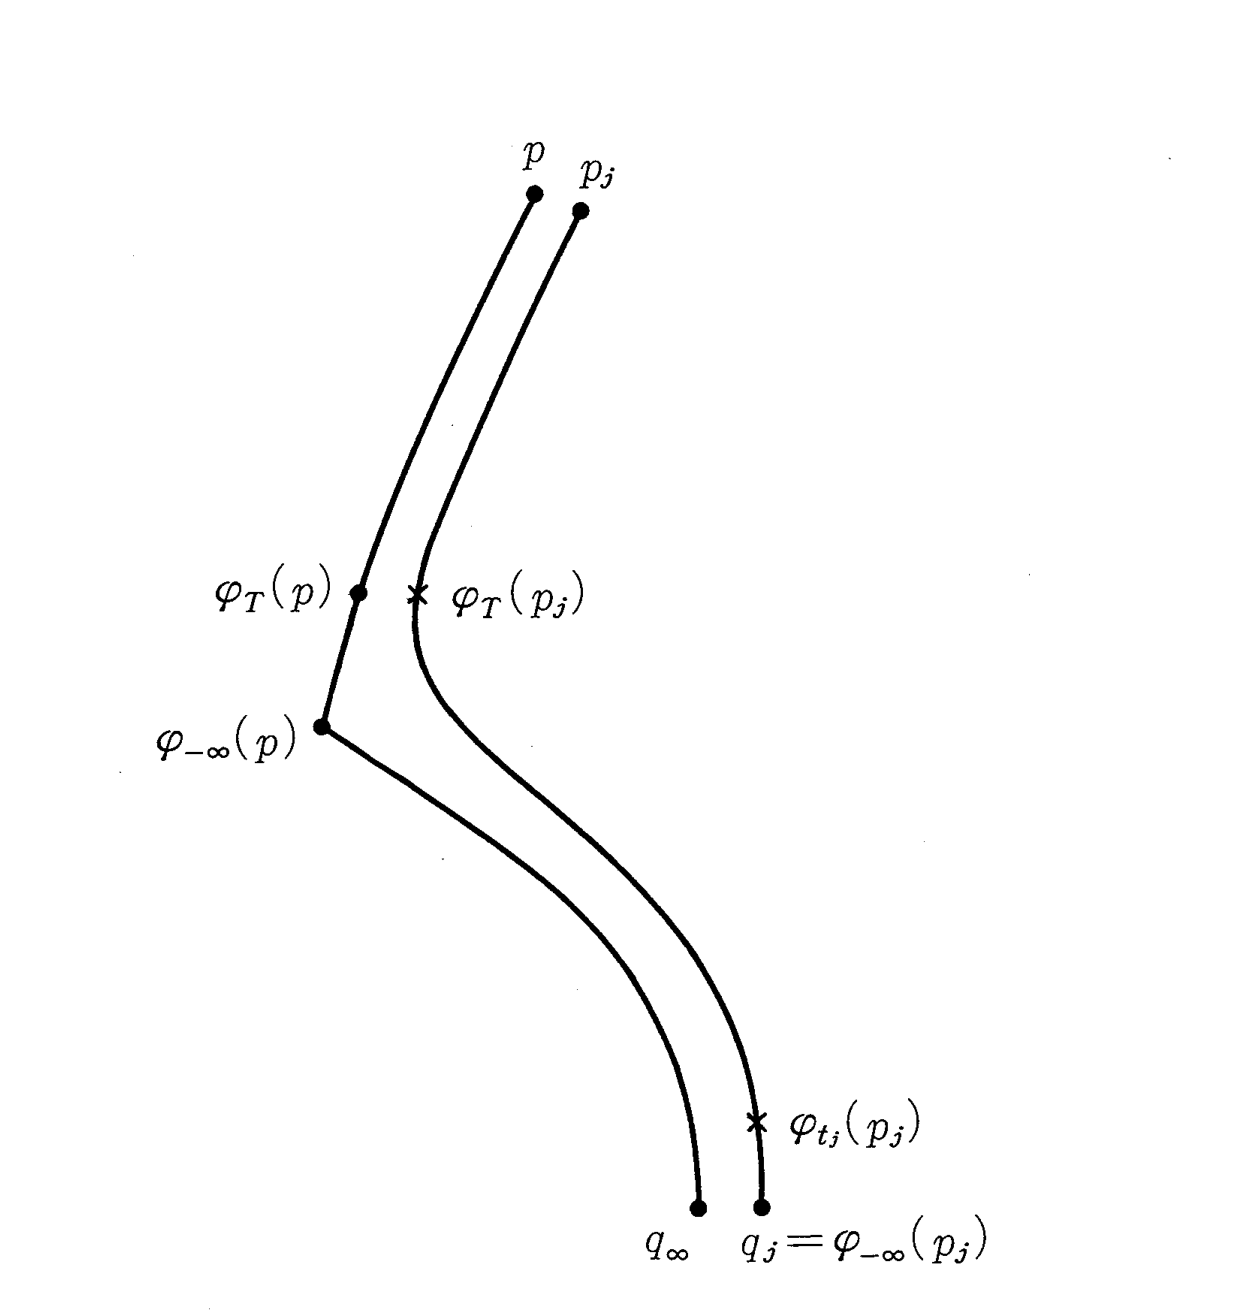
\includegraphics[width=0.52\textwidth]{figures/fig3.1.png}
  \figtitle{3.1}{梯度向量场的轨道分裂（原书 p.94）}
\end{figure}

因此，不妨认为 $\mathfrak{X}_i(M)$ 是 $M$ 的某个三角形剖分的子复形。于是得到奇异链复形 $S_*(M)$ 的滤过（filtration）
\[
  S_*(\mathfrak{X}_0(M))\subset S_*(\mathfrak{X}_1(M))\subset\cdots\subset S_*(\mathfrak{X}_J(M))=S_*(M)
\]
（$S_*(X)$ 是空间 $X$ 的奇异链复形）。由此得到收敛到 $S_*(M)$ 的同调的谱序列。其 $E^2$ 项是
\begin{equation}
  \bigoplus_iH_*(\mathfrak{X}_i(M),\mathfrak{X}_{i-1}(M)). \tag{3.13}
\end{equation}
由切除同型与引理 3.18，(3.13) 与 $\bigoplus_iH_k(N_i^{+},N_i^{+}-R_i;\Z)$ 同型。
\end{proof}

同调群 $H_k(N_i^{+},N_i^{+}-R_i;\Z)$，在向量丛 $N_i^{+}$ 可定向时，等于 $H_{k+\mu(R_i)+\dim R_i-n}(R_i;\Z)$。

这称为 \textbf{Thom 同型}（Thom isomorphism）。又，$N_i^{+}$ 的秩是 $n-\mu(R_i)-\dim R_i$。

当 $f$ 是动量映射时，$N_i^{+}$ 的每个纤维上确定有不带不动点的 $S^1$ 作用。利用这一点可知 $N_i^{+}$ 可定向。进一步可知下面的事实。

% [Tutor Note: “$N_i^{+}$ 的纤维上有不带不动点的 $S^1$ 作用”来自 §3.2 开头的表示分解：纤维方向按权重 $\lambda$ 分解，而 $N_i^{+}$ 对应正权重部分。不动点集为空正是“正权重”的几何含义；由此可给 $N_i^{+}$ 定向，进而用 Thom 同型把相对同调换成 $R_i$ 的同调。]

% [原文 p.95]
\begin{theorem}{3.23}
  当 $f$ 是动量映射时，定理 3.17 的谱序列在 $E^2$ 项退化。即
  \[
    H_k(M;\Z)\cong\bigoplus_iH_{k+\mu(R_i)+\dim R_i-n}(R_i;\Z).
  \]
\end{theorem}

若 $M$、$R_i$ 可定向，用 Poincaré 对偶，定理 3.23 就成为
\[
  H^k(M;\Z)\cong\bigoplus_iH^{k-\mu(R_i)}(R_i;\Z).
\]
（次数的约定是为了变成上同调时看起来自然，故定理 3.23 右端的次数 $k+\mu(R_i)+\dim R_i-n$ 看起来不自然。）

用等变上同调给出的定理 3.23 的证明将在 §3.4 叙述。§5.3 将给出无限维情形（例 3.10）也适用的另一证明。

\begin{definition}{3.24}
  使定理 3.23 的结论成立的 Bott–Morse 函数称为\textbf{完全 Bott–Morse 函数}（perfect Bott–Morse function）。
\end{definition}

作为定理 3.23 的应用，来证明下面的定理（据 Atiyah [18]、Guillemin–Sternberg [166]）。设连通紧可换群 $G$ 在 $(M,\omega)$ 上有哈密顿作用，$f\colon M\to\mathfrak{g}^*$ 是动量映射。

\begin{theorem*}{3.25}
  若 $M$ 连通且紧，则 $f$ 的像 $f(M)$ 是凸集。
\end{theorem*}

\begin{proof}
  不妨假定 $G$ 的作用是有效的（effective，即若对所有的 $x\in M$ 都有 $g\cdot x=x$，则 $g=1$）。

  把 $f(M)$ 在 $\mathfrak{g}^*$ 中的内点全体之集记作 $f(M)^\circ$。先证 $f(M)^\circ$ 的闭包与 $f(M)$ 一致。由作用有效可知，满足 $G_x=1$ 的点 $x$ 全体在 $M$ 中稠密。另一方面，$G$ 可换，故动量映射是 $G$ 不变的。

  当 $G_x=1$ 时，证明 $d_xf\colon T_xM\to T_{f(x)}\mathfrak{g}^*=\mathfrak{g}^*$ 是满射。若不然，则存在 $W\in\mathfrak{g}$ 使 $(d_xf)(V)(W)=0$ 对任意的 $V\in\mathfrak{g}$ 成立。（这里用 $G$ 的作用把 $V\in\mathfrak{g}$ 看作 $T_xM$ 的元素。）于是由定义 3.1 (1)，$\omega(W,V)=0$。故由 $\omega$ 非退化得 $W(x)=0$。另一方面，由 $G_x=1$ 知 $\mathfrak{g}\to T_xM$ 是单射，矛盾。
\end{proof}

% [原文 p.96]
\begin{proof}[证明（续）]
因此，若 $G_x=1$，则 $f(x)$ 是 $f(M)$ 的内点。由此可知 $f(M)^\circ$ 在 $f(M)$ 中稠密。

所以，要证 $f(M)$ 是凸的，只需证明：对任意的 $\alpha\in E^*$，使 $\alpha$ 在 $K$ 上的限制取极小的点全体之集连通。这里 $V^*$ 表示对偶空间，$\mathfrak{g}^*$ 的对偶空间是 $\mathfrak{g}$。取 $V\in\mathfrak{g}$，考虑函数 $f_V(p)=f(p)(V)$。只需证明使 $f_V$ 取极小的点全体之集连通。

% [Tutor Note: 原书 p.96 此句作“对任意的 $\alpha\in E^*$，使 $\alpha$ 在 $K$ 上的限制取极小……”，其中 $E^*$、$K$ 疑为 $\mathfrak{g}^*$、$f(M)$ 之误植：凸性判据要求对每个线性泛函 $\alpha\in(\mathfrak{g}^*)^*=\mathfrak{g}$，考察 $\alpha$ 在凸集 $f(M)$ 上的极小点集是否连通。作者随即转到 $V\in\mathfrak{g}$ 与 $f_V$，正好与这一读法一致。]

$\{\exp(tV)\mid t\in\R\}$ 在 $G$ 中的闭包是 $G$ 的子群（$\exp(tV)$ 是李群的指数映射）。把 $V$ 作小幅变动，不妨设这个群是 $S^1$。（若 $f_V$ 取极小的点全体之集不连通，则 $V$ 作小幅变动后同一性质仍成立（图 3.2）。）

\begin{figure}[htbp]
  \centering
  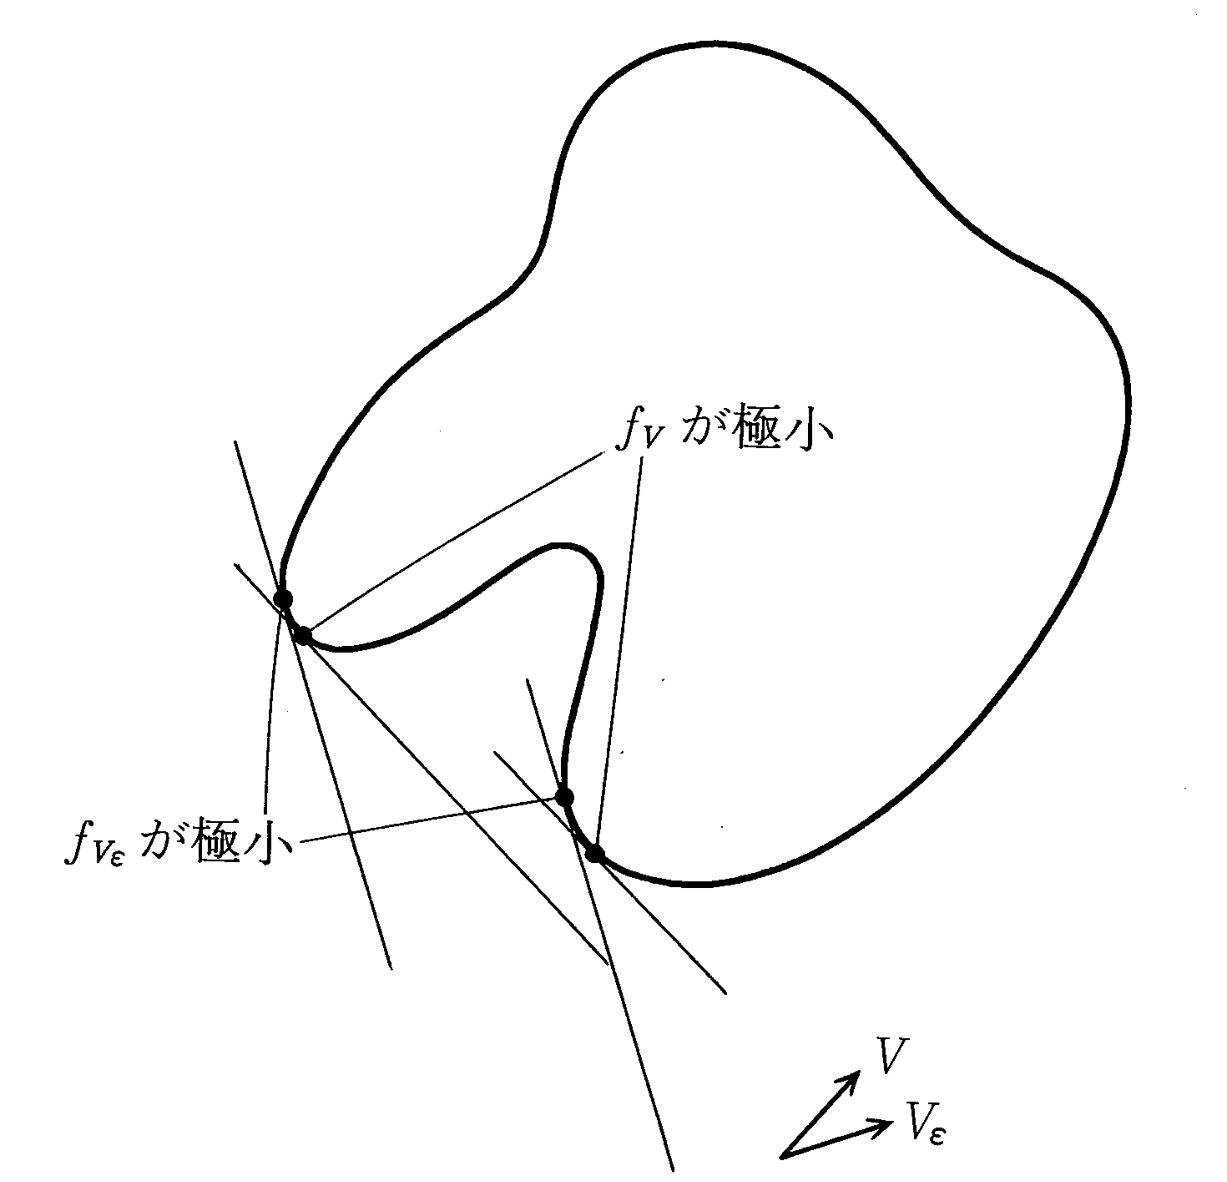
\includegraphics[width=0.50\textwidth]{figures/fig3.2.png}
  \figtitle{3.2}{变动 $V$（原书 p.96）}
\end{figure}

于是 $f_V$ 是关于这个 $S^1\subset G$ 的作用的动量映射。故由定理 3.23，
\[
  H_0(M;\Z)\cong\bigoplus_{\mu(R_i)=0}H_0(R_i;\Z).
\]
因此使 $\mu(R_i)=0$ 的 $i$ 只有一个。另一方面，使 $f_V$ 取极小的点全体之集与 $\mu(R_i)=0$ 的 $R_i$ 的并集一致。
\end{proof}

% [原文 p.97]
\section{与复几何的关系}

\takeaway{在凯勒流形上，保持复结构的哈密顿 $G$-作用可以“复化”为复李群 $G_{\C}$ 的全纯作用：$g=\exp(X)k$ 对应 $\exp(J_MY)$ 与 $k$ 的复合。由此辛商 $f^{-1}(0)/G$ 同时是复流形 $M/\!/G_{\C}$，二者在凯勒情形给出同一个空间。}

本节叙述复流形 $M$ 关于复李群 $G_{\C}$ 的商空间与辛商的关系。考虑复李群的商时最大的问题在于：复李群极少是紧的。事实上已知紧复李群只限于可换群（环面）（例如参见 [270]）。若 $M$ 紧而 $G_{\C}$ 不紧，则按通常想法得到的商空间 $M/G_{\C}$ 不是 Hausdorff 空间。因此不能采取“先取商空间、再在商空间上放复结构”这种造法。Mumford [269]、[271] 的想法大略是：从 $M$ 中除去称为不稳定点的点集 $M_{us}$，考虑 $M_{ss}=M-M_{us}$ 关于 $G_{\C}$ 作用的商空间 $M_{ss}/G_{\C}$，这样就能得到复流形。本节说明：在凯勒流形的情形，这一构造与辛商的构造一致。从下述状况出发。

\begin{definition}{3.26}
  \textbf{复李群} $G_{\C}$ 是指复流形 $G_{\C}$ 连同全纯映射 $\cdot\colon G\times G\to G$、$^{-1}\colon G\to G$ 与元素 $1\in G$，它们使 $G$ 上确定群结构。复李群 $G_{\C}$ 在复流形 $M$ 上的作用，是指确定作用的映射 $G\times M\to M$ 是全纯映射。
\end{definition}

\begin{assumption}{3.27}
  $G_{\C}$ 是复李群，$G$ 是它的李子群，且满足下列性质。

  (1) $G$ 是紧的。

  (2) $JT_1G\cap T_1G=\{0\}$，且 $JT_1G+T_1G=T_1G_{\C}$。这里 $1\in G$ 是单位元。

  (3) 对任意的 $g\in G_{\C}$，存在唯一的 $k\in G$ 与 $X\in JT_1G$，使 $g=\exp(X)k$ 成立。
\end{assumption}

\begin{definition}{3.28}
  称 $G$ 为 $G_{\C}$ 的\textbf{紧实形式}（compact real form）。
\end{definition}

% [Tutor Note: 假定 3.27 (2)、(3) 中的 $J$ 是 $G_{\C}$ 上的复结构（左不变），$T_1G_{\C}$ 与 $T_1G$ 分别是两个群在单位元处的切空间。条件 (2) 说的是 $T_1G_{\C}$ 恰是 $T_1G$ 与其 $J$ 像的实直和；(3) 则是说每个 $g$ 可唯一地写成 $G$ 中元素与 $\exp(JT_1G)$ 中元素的乘积，即极分解。]

例如，若 $G_{\C}$ 半单，则已知总存在满足假定的 $G$。举几个例子。

\begin{example}{3.29}
  设 $G_{\C}=\C^{*n}$（$\C^*=\C-\{0\}$）。此时 $G=T^n=\{(z_1,\dots,z_n)\mid|z_i|=1\}$。
\end{example}

% [原文 p.98]
\begin{example}{3.30}
  设 $G_{\C}=SL(n;\C)$，即行列式为 1 的复矩阵全体。置
  \[
    SU(n)=\{k\mid{}^t\bar k=k^{-1}\},\qquad
    E^{+}(n)=\{h\mid{}^t\bar h=h,\ \forall v\in\C^n,\ hv\cdot v>0\}.
  \]
  则对任意的 $g\in SL(n;\C)$，存在唯一的分解 $g=hk$，$g\in SU(n)$，$h\in E^{+}(n)$。又对 $h\in E^{+}(n)$，存在唯一的 Hermite 矩阵 $X$ 使 $h=\exp X$。$g=\exp(X)k$ 就是所求的分解。
\end{example}

设 $(M,J_M,\omega_M)$ 是凯勒流形。考虑保持复结构与辛结构的群 $G$ 在 $(M,\omega_M)$ 上的作用。这里，$G$ 在 $(M,\omega_M)$ 上的作用保持复结构，是指对任意的 $g\in G$，它所确定的映射 $g\colon M\to M$ 是全纯映射。

从这一点出发，来构造 $G_{\C}$ 在 $(M,J_M)$ 上作为复李群的作用。设 $g\in G_{\C}$，按假定 3.27 分解为 $g=\exp(X)k$。令 $Y=-\sqrt{-1}X\in\mathfrak{g}$，置
\begin{equation}
  g\cdot p=\exp(J_MY)(k\cdot p) \tag{3.14}
\end{equation}
（$\exp(tJ_MY)$ 表示向量场 $J_MY$ 生成的 1 参数变换群）。

\begin{proposition*}{3.31}
  (3.14) 确定 $G_{\C}$ 在 $(M,J_M)$ 上作为复李群的作用。
\end{proposition*}

\begin{proof}
  首先看 (3.14) 给出群作用，即对 $g_1,g_2\in G_{\C}$ 有 $(g_1g_2)x=g_1(g_2x)$。为此，只需证明映射 $\mathfrak{g}\otimes\C\to\Gamma(TM)$，$X+\sqrt{-1}Y\mapsto X+J_M(Y)$ 是李代数的同态。由于 $G$ 在 $M$ 上的作用保持复结构，李导数 $L_XJ_M$、$L_YJ_M$ 为 0。即 $[J_MX,V]=J_M([X,V])$ 等成立。利用这一点可以验证 $X+\sqrt{-1}Y\mapsto X+J_M(Y)$ 是李代数的同态。

  其次，固定一点 $p\in M$ 时，映射 $g\mapsto g\cdot p$，$G\to M$ 是全纯映射（这由定义显然）。因此，要证映射 $G\times M\to M$，$(g,p)\mapsto g\cdot p$ 是全纯映射，只需对固定的 $X\in\mathfrak{g}$ 证明 $p\mapsto\exp(J_MX)(p)$，$M\to M$ 是全纯映射。换言之，只需证 $L_{J_MX}J_M=0$。
\end{proof}

% [Tutor Note: 原书 p.98 把群作用的条件印作 $g_1(g_2x)=g_1(g_2x)$，左右两端相同，显然是 $(g_1g_2)x=g_1(g_2x)$ 之误，此处按此写。另注意 (3.14) 的两步：先用 $k\in G$（保复结构），再用 $\exp(J_MY)$；$Y=-\sqrt{-1}X$ 中的 $\sqrt{-1}$ 来自“把 $X\in\mathfrak{g}$ 复化为 $\mathfrak{g}\otimes\C=T^{1,0}\oplus T^{0,1}$ 中的 $(0,1)$ 分量”。]

% [原文 p.99]
把 $X$ 分解为 $X=X_{1,0}+X_{0,1}$，按 $TM\otimes\C=T^{1,0}M\oplus T^{0,1}M$ 进行。由于 $G$ 的作用保持复结构，$\operatorname{ad}X$ 保持 $T^{1,0}M\subset TM\otimes\C$。另一方面 $J_M$ 可积，故 $[\Gamma(T^{1,0}),\Gamma(T^{1,0})]\subset\Gamma(T^{1,0})$，$[\Gamma(T^{0,1}),\Gamma(T^{0,1})]\subset\Gamma(T^{0,1})$。设 $Y\in\Gamma(T^{1,0})$，则 $[X_{0,1},Y]=[X,Y]-[X_{1,0},Y]\in\Gamma(T^{1,0})$。因此
\[
  [J_MX,Y]=[J_MX_{1,0},Y]+[J_MX_{0,1},Y]
  =[\sqrt{-1}X_{1,0},Y]-[\sqrt{-1}X_{0,1},Y]\in\Gamma(T^{1,0}).
\]
即 $L_{J_MX}J_M=0$。

以上，由 $(M,J_M,\omega_M)$ 上保持复结构的哈密顿作用，确定了 $G_{\C}$ 在 $(M,J_M)$ 上作为复李群的作用。这个构造有逆。

\begin{lemma*}{3.32}
  设 $(M,J_M,\omega_M)$ 是凯勒流形，复李群 $G_{\C}$ 作用其上。此时，必要时把凯勒度量 $\omega_M$ 换掉，取另一个凯勒度量 $\omega'_M$，则 $(M,J_M,\omega'_M)$ 是凯勒流形，且 $G$ 的作用保持 $\omega'_M$。若 $G$ 的作用是哈密顿作用，则 $G_{\C}$ 的作用由式 (3.14) 得到。
\end{lemma*}

\begin{proof}
  $\omega'_M$ 可这样得到：把 $\omega_M$ 经 $G$ 的作用变动所得的微分 2 形式们，关于 $G$ 的双边不变测度取平均。证明的其余部分，把命题 3.31 的证明中的计算倒过来追溯即可。
\end{proof}

其次假定群 $G$ 的作用是哈密顿作用，设 $f\colon M\to\mathfrak{g}^*$ 为动量映射。

\begin{proposition*}{3.33}
  $f^{-1}(x)$ 的 $G_{\C}$ 轨道 $G_{\C}\cdot f^{-1}(x)$ 是 $M$ 的稠密子集。
\end{proposition*}

\begin{proof}
  考虑函数 $h(x)=\|f(x)\|^2$。\footnote{$h$ 的 Morse 理论将在下一节详论。}这里 $\|\ \|$ 是 $\mathfrak{g}^*$ 的 $G$ 不变内积。$\|\ \|$ 是 $G$ 不变的，故 $h$ 也是 $G$ 不变的。

  以下用定义 $\|\ \|$ 所用的 $G$ 不变内积 $\langle\cdot,\cdot\rangle$ 把 $\mathfrak{g}$ 与 $\mathfrak{g}^*$ 等同起来。设 $x\in M$，置 $W=f(x)$。把 $W$ 看作 $\mathfrak{g}$ 的元素，再把它看作 $T_xM$
% [原文 p.100]
  的元素。此时对 $V\in T_xM$ 有
\[
  dh(V)=2df(V)(W)=2\omega_M(W,V)=2\langle J_MW,V\rangle
\]
成立。即 $\operatorname{grad}_xh=2J_MW$。因此 $\operatorname{grad}_xh$ 的积分曲线含于 $G_{\C}$ 的轨道之中。又 $G_{\C}\cdot f^{-1}(0)$ 含有 $f^{-1}(0)$ 的某个充分小邻域的稠密子集。因此，只需证明 $h$ 没有 0 以外的极小值。设 $h$ 在 $x$ 处取极小，$f(x)=W$。置 $h'(y)=f(y)(W)$，则 $\{y\mid h'(y)\ge h'(x)\}$ 含于 $\{y\mid h(y)\ge h(x)\}$。故 $h'$ 在 $x$ 处取极小，但这与定理 3.23 矛盾。
\end{proof}

由命题 3.33，辛商 $f^{-1}(0)/G$ 就是把 $M$ 的稠密开子集 $G_{\C}\cdot f^{-1}(0)$ 用复李群 $G_{\C}$ 的作用除得的商。这个空间也写作 $M/\!/G_{\C}$。由于 $G$ 紧，商空间 $M/\!/G_{\C}$ 是 Hausdorff 空间。由第一个描述 $M/\!/G_{\C}=f^{-1}(0)/G$ 可知 $M/\!/G_{\C}$ 上有辛结构；由第二个描述 $M/\!/G_{\C}=G_{\C}\cdot f^{-1}(0)/G_{\C}$ 可知 $M/\!/G_{\C}$ 上有复结构。

\begin{lemma}{3.34}
  $M/\!/G_{\C}$ 是凯勒流形。
\end{lemma}

证明很容易。

% [Tutor Note: 这里“两个描述”指的是把同一个空间分别看成 $f^{-1}(0)/G$ 与 $G_{\C}\cdot f^{-1}(0)/G_{\C}$。前一个描述给辛结构、后一个给复结构，二者相容即凯勒结构；命题 3.33 的稠密性是这两个描述能粘合的关键。]

称 $G_{\C}\cdot f^{-1}(0)$ 的点为\textbf{稳定}（stable）点，其余的点为\textbf{不稳定}（unstable）点。\footnote{代数几何中半稳定（semistable）这一概念也很重要。本书的用语与代数几何的用语略有出入。}

在代数几何中，上述构造如下出现。设 $G_{\C}\subset GL(n+1;\C)$，$G=G_{\C}\cap U(n+1)$，且 $G$ 是 $G_{\C}$ 的紧实形式。设 $P_1,\dots,P_k$ 是 $n+1$ 个变元的齐次多项式，由 $P_i$ 们生成的 $\C[z_0,\dots,z_n]$ 的理想（ideal）关于 $G_{\C}$ 不变。用粗体字母如 $\bm z$ 表示 $\C^{n+1}$ 的点。对 $\bm z\neq0$，把对应的 $\CP^n$ 的点写作 $[\bm z]$。假定 $M=\{[\bm z]\mid P_i(\bm z)=0\}\subset\CP^n$ 是光滑流形。$G$、$G_{\C}$ 作用在 $M$ 上，且 $G$ 保持 $M$ 的凯勒形式。

$\C^{n+1}$ 的凯勒度量 $\langle\cdot,\cdot\rangle$ 与凯勒形式 $\omega$ 是

% [原文 p.101]
\[
  \langle\bm z,\bm w\rangle=\sum_i\operatorname{Re}(z_i\bar w_i),\qquad
  \omega(\bm z,\bm w)=\sum_i\operatorname{Im}(z_i\bar w_i)
\]
设 $(n+1)\times(n+1)$ 矩阵 $A$ 是 $G$ 的李代数的元素。利用 ${}^t\bar A=-A$ 可以验证 $\omega(AX,Y)=\omega(AY,X)$。

\begin{proposition*}{3.35}
  $G$ 在 $M$ 上的作用的动量映射由下式给出的 $f$ 给出：
  \[
    f([\bm z])=\frac{\omega(A\bm z,\bm z)}{2\langle\bm z,\bm z\rangle}.
  \]
\end{proposition*}

\begin{proof}
  设 $\bm z(t)$ 是满足 $\|\bm z(t)\|=1$、$\bm z(0)=\bm z$、$P(\bm z(t))=0$ 的道路，置 $d\bm z/dt(0)=V$。设 $\pi\colon\C^{n+1}\setminus\{0\}\to\CP^n$ 为射影。$A\in\mathfrak{g}$ 确定 $T_{[\bm z]}\CP^n$ 的元素，这个元素就是 $(d\pi)(A\bm z)$。另一方面，
  \begin{align*}
    \frac{d}{dt}f([\bm z(t)])\Big|_{t=0}(A)
    &=\frac{1}{2}\frac{d}{dt}\omega(A\bm z(t),\bm z(t))\Big|_{t=0}
     =\frac{1}{2}\bigl(\omega(AV,\bm z)+\omega(A\bm z,V)\bigr)\\
    &=\omega(A\bm z,V)=\omega_M\bigl((d\pi)(A\bm z),(d\pi)(V)\bigr).
  \end{align*}
  这意味着定义 3.1 (1)。(2) 的证明容易。
\end{proof}

\begin{proposition*}{3.36}
  $[\bm z]\in G_{\C}\cdot f^{-1}(0)$ 与 $0\notin\overline{G_{\C}\cdot\bm z}$ 等价。
\end{proposition*}

\begin{proof}
  设 $0\notin\overline{G_{\C}\cdot\bm z}$。在 $G_{\C}\cdot\bm z$ 中存在离 $0$ 最近的元素 $g\bm z$。置 $\bm w=g\bm z/\|g\bm z\|$，则由命题 3.35 与 $\omega(A\bm z,\bm z)=\langle\sqrt{-1}\bm z,\bm z\rangle$ 可知 $f([\bm w])=0$。因此 $g^{-1}([\bm w])=[\bm z]$，$\bm w\in f^{-1}(0)$。

  反之设 $f([\bm z])=0$。由命题 3.35，$g\mapsto\|g\bm z\|$ 在 $g=1$ 处取极值。容易看出极值只能是极小值，故 $g\mapsto\|g\bm z\|$ 在 $g=1$ 处取最小。因此 $\|g\bm z\|\ge\|\bm z\|\ge c>0$。即 $0\notin\overline{G_{\C}\cdot\bm z}$。
\end{proof}

$0\notin\overline{G_{\C}\cdot\bm z}$ 就是代数几何中（半）稳定性的定义（参见 [269]、[268]）。

\begin{example}{3.37}
  把对角成分为 $a,b,c$ 的 $3\times3$ 矩阵写作 $\operatorname{mat}(a,b,c)$。置 $M=\CP^2$，$G=\{\operatorname{mat}(a,b,(ab)^{-1})\mid|a|=|b|=1\}\cong T^2$，$G_{\C}=\{\operatorname{mat}(a,b,(ab)^{-1})\mid a,b\in\C^*\}$。$G_{\C}$ 有效作用在 $M$ 上。取 $A_1=(\sqrt{-1},0,-\sqrt{-1})$，$A_2=(0,\sqrt{-1},-\sqrt{-1})$ 为 $G$ 的李代数的生成元。
\end{example}

% [原文 p.102]
\begin{equation}
  \begin{aligned}
    f([z_0:z_1:z_2])(A_1)&=\frac{|z_0|^2-|z_2|^2}{2(|z_0|^2+|z_1|^2+|z_2|^2)^2},\\
    f([z_0:z_1:z_2])(A_2)&=\frac{|z_1|^2-|z_2|^2}{2(|z_0|^2+|z_1|^2+|z_2|^2)^2}.
  \end{aligned}
  \tag{3.15}
\end{equation}
因此 $f^{-1}(0)=\{[z_0:z_1:z_2]\mid|z_0|=|z_1|=|z_2|\neq0\}\cong T^2$。$[z_0:z_1:z_2]$ 为不稳定点与 $z_0z_1z_2=0$ 等价。

如前所述，动量映射或辛商并不唯一。从第二个描述 $G_{\C}\cdot f^{-1}(0)/G_{\C}$ 的立场看，这是集合 $G_{\C}\cdot f^{-1}(x)$ 随 $x$ 而变的归结。也就是说，稳定性的定义随动量映射的取法而变化。下面在 $G=S^1$ 的情形考察这一状况。

考虑梯度向量场 $\operatorname{grad}f$。设 $\varphi_t$ 是 $\operatorname{grad}f$ 生成的 1 参数变换群。由 (3.14)，$\C^*f^{-1}(x)=\{\varphi_t(p)\mid f(p)=x,\ t\in\R\}$。

设 $\operatorname{Cr}(f)=\bigcup_iR_i$ 是到连通分量的分解，使用定理 3.17 证明中的记号。$\dim U(R_i)=\mu(R_i)+\dim R_i$ 等于 $p\in R_{i,j}$ 处 $\operatorname{Hess}_pf$ 的非负特征值的个数，$\dim S(R_i)$ 等于 $p\in R_i$ 处 $\operatorname{Hess}_pf$ 的非正特征值的个数。

% [Tutor Note: 原书 p.102 此处作 $p\in R_{i,j}$，指标 $j$ 在全书他处并未出现，应为 $p\in R_i$。又“非负特征值个数”含 0 特征值，故 $\dim U(R_i)$ 比“不稳定流形维数 = 正特征值个数”多出 $\dim R_i$，这正是 $\mu(R_i)+\dim R_i$ 的来源。]

设 $x_0\in\R$ 是临界值。不妨设 $f^{-1}(x_0)$ 所含临界点之集连通，记为 $R_i$。把 $\C^*\cdot f^{-1}(x_0-\epsilon)$ 写作 $X_-$，$\C^*\cdot f^{-1}(x_0+\epsilon)$ 写作 $X_+$（$\epsilon$ 是充分小的正数）。此时 $X_+-S(R_i)\simeq X_--U(R_i)$ 成立。考虑 $R_i$ 上两个向量丛 $N_-R_i$ 与 $N_+R_i$。它们分别与 $S(R_i)$ 和 $U(R_i)$ 微分同胚。它们关于 $S^1$ 或更一般地关于 $\C^*$ 的作用不变。$(N_-R_i-R_i)/\C^*$、$(N_+R_i-R_i)/\C^*$ 是以 $R_i$ 上的复射影空间为纤维的纤维丛，是复流形。
\[
  f^{-1}(x_0-\epsilon)/S^1-(N_-R_i-R_i)/\C^*=f^{-1}(x_0+\epsilon)/S^1-(N_+R_i-R_i)/\C^*
\]
由此可知，从 $f^{-1}(x_0-\epsilon)/S^1$ 作出 $f^{-1}(x_0+\epsilon)/S^1$ 的操作，是称为翻转（flip）或 flop 的操作之一例（关于这些，参见 [263]）。

代数几何中的稳定性及其与不变量理论的关系，[268] 中有详述，请读者参看那里。本节构造的具体例中属于代数几

% [原文 p.103]
何的，[268] 中会有解说。

因此，下面举一个种类稍异的例子。回想例 3.10。那里对黎曼面 $\Sigma$ 上向量丛 $E$ 的联络全体之空间考虑了辛结构，看到规范变换群的作用是哈密顿作用，辛商是平坦联络的模空间。到此为止的构造没有用到黎曼面 $\Sigma$ 的复结构。

取 $\Sigma$ 的复结构 $J_\Sigma$。又设复李群 $G_{\C}$ 是紧李群 $G$（$E$ 的结构群）的复化。换言之，设 $G\subset G_{\C}$ 满足假定 3.27。已知可以取 $G_{\C}\subset GL(n;\C)$，$G=G_{\C}\cap U(n)$。（参见李群论的书籍。在 $G=U(n),SU(n)$，$G_{\C}=GL(n;\C),SL(n;\C)$ 等情形是明显的。）

联络空间 $\mathcal{A}(\Sigma,E)$ 在一点 $A$ 处的切空间是 $\Gamma(\Sigma;\mathrm{Ad}\,E\otimes_{\R}\Lambda^1)$。$J_\Sigma$ 引起 $\Lambda^1$ 到自身的映射 $J_\Sigma$。考虑凯勒度量 $g_\Sigma$，设其 Hodge 算子为 $*_\Sigma$，则 $J_\Sigma=*_\Sigma$。换言之，$u\wedge J_\Sigma v=g_\Sigma(u,v)\Omega_\Sigma$ 成立。特别地 $J_\Sigma J_\Sigma=-1$。赋以这个（近）复结构的 $\mathcal{A}(\Sigma,E)$ 与无限维复向量空间同构，故 $J_\Sigma$ 可积。

由于 $-\operatorname{Tr}$ 是 $\mathfrak{g}$ 上的不变正定内积，
\[
  \omega(V,J_\Sigma V)=-\frac{1}{8\pi^2}\int_\Sigma\operatorname{Tr}(V\wedge*_\Sigma V)\ge0
\]
成立。即 $g_\Sigma(V,W)=\omega(V,J_\Sigma W)$ 确定 $\mathcal{A}(\Sigma,E)$ 上的凯勒度量。

那么，规范变换群 $\mathcal{G}(\Sigma,E)$ 是 $G$ 值的“函数”（$E$ 有扭折，故与函数略有不同）。这个群是无限维的，故不紧，但它是取值于紧群的映射之集，故具有与紧群许多共同的性质。可以把这个群看作本节所论的 $G$。$\mathcal{G}(\Sigma,E)$ 保持辛结构 $\omega$ 一事已经说过，而它保持复结构 $J_\Sigma$。因此我们大致处于命题 3.31 的状况。$\mathcal{G}(\Sigma,E)$ 的复化是 $G_{\C}$ 值规范变换全体。记作 $\mathcal{G}_{\C}(\Sigma,E)$

% [原文 p.104]
吧。

来计算 $\mathcal{G}_{\C}(\Sigma,E)$ 在 $\mathcal{A}(\Sigma,E)$ 上的作用。取定 $\mathcal{A}(\Sigma,E)$ 的元素 $\nabla_0$，把 $\mathcal{A}(\Sigma,E)$ 的元素 $\nabla$ 对应到 $A=\nabla-\nabla_0$，从而把 $\mathcal{A}(\Sigma,E)$ 与 $\Gamma(\Sigma;\mathrm{Ad}\,E\otimes\Lambda^{0,1})$ 等同起来。由 $\mathfrak{g}\subset\mathfrak{u}(n)$ 得 ${}^t\bar A=-A$。

考虑 $d_Ag=\nabla_0g+[A,g]$，用 $\Sigma$ 的复结构把它分解为 $d_Ag=\partial_Ag+\bar\partial_Ag$。这里 $\partial_Ag$ 是 $\Gamma(\Sigma;\mathrm{Ad}\,E\otimes\Lambda^{1,0})$ 的元素，$\bar\partial_Ag$ 是 $\Gamma(\Sigma;\mathrm{Ad}\,E\otimes\Lambda^{0,1})$ 的元素。

\begin{proposition*}{3.38}
  (3.14) 的作用由 (3.16) 给出。
  \begin{equation}
    g^*A=g\bar\partial_Ag^{-1}+{}^t\bar g^{-1}\partial_A{}^t\bar g. \tag{3.16}
  \end{equation}
\end{proposition*}

\begin{proof}
  只需证明 (3.16) 给出 $\mathcal{G}_{\C}(\Sigma,E)$ 在 $\mathcal{A}(\Sigma,E)$ 上作为复李群的作用，且它在 $\mathcal{G}(\Sigma,E)$ 上与普通的规范变换一致。

  来证后者。设 $g\in\mathcal{G}(\Sigma,E)$，则 ${}^t\bar g=g^{-1}$，故
  \[
    g\bar\partial_Ag^{-1}+{}^t\bar g^{-1}\partial_A{}^t\bar g=g\bar\partial_Ag^{-1}+g\partial_Ag^{-1}=gd_Ag^{-1}.
  \]
  为证前者，先把 (3.16) 的作用改写。$\mathrm{Ad}\,E$ 的纤维是 $\mathfrak{g}$，其复化 $\mathfrak{g}\otimes\C$ 是 $G_{\C}$ 的李代数 $\mathfrak{g}_{\C}$。$\mathrm{Ad}\,E_{\C}=\mathrm{Ad}\,E\otimes\C$ 是以 $\mathfrak{g}_{\C}$ 为纤维的向量丛。来构造同型
  \begin{equation}
    \mathrm{Ad}\,E\otimes_{\R}\Lambda^1\simeq\mathrm{Ad}\,E_{\C}\otimes_{\C}\Lambda^{0,1} \tag{3.17}
  \end{equation}
  （这里 $\Lambda^1$ 是实值微分 1 形式全体）。首先 $\mathrm{Ad}\,E\otimes_{\R}\Lambda^1\subset(\mathrm{Ad}\,E\otimes_{\R}\Lambda^1)\otimes\C$。分解 $\Lambda^1\otimes\C=\Lambda^{1,0}\oplus\Lambda^{0,1}$。其射影确定 $(\mathrm{Ad}\,E\otimes_{\R}\Lambda^1)\otimes\C\to\mathrm{Ad}\,E_{\C}\otimes_{\C}\Lambda^{0,1}$。这两个映射的合成就是 (3.17)。$J_\Sigma$ 在 $\Lambda^{0,1}$ 上以 $-\sqrt{-1}$ 倍作用，故 (3.17) 是反复线性的。
\end{proof}

\begin{remark}{3.39}
  $G=U(n)$ 时的 (3.17) 表达了这样一件熟知的事实：给定向量丛上的复结构，就唯一存在与它相容的酉联络。
\end{remark}

把 (3.17) 的同型具体写出。把 $A\in\mathrm{Ad}\,E\otimes_{\R}\Lambda^1$ 分解为 1,0 成分与 0,1 成分：$A=A^{1,0}+A^{0,1}$，则 $A\mapsto A^{0,1}$ 是从左端到右端的映射。

\begin{proof}[证明（续）]

% [原文 p.105]
计算其逆。首先注意 $\mathfrak{g}_{\C}$ 中的复共轭由 $A\mapsto-{}^t\bar A$ 给出（由 $\mathfrak{g}$ 的元素满足 $-{}^t\bar A=A$ 可知）。因此 (3.17) 的右端到左端的映射由
\begin{equation}
  A^{0,1}\mapsto-{}^t\bar A^{0,1}+A^{0,1} \tag{3.18}
\end{equation}
给出。那么，对 $A^{0,1}\in\mathrm{Ad}\,E_{\C}\otimes_{\C}\Lambda^{0,1}$ 置
\begin{equation}
  g^*A^{0,1}=g\bar\partial_{A^{0,1}}g^{-1}. \tag{3.19}
\end{equation}
比较定义便知，把 (3.19) 经 (3.18) 搬运过去就是 (3.16)。

要证 (3.16) 给出保复结构的作用，只需证 (3.19) 是保复结构的作用（两个反复线性映射与复线性映射的合成是复线性的）。定义映射 $\bar\partial_{A^{0,1}}\colon\Gamma(\Sigma;E\otimes\C)\to\Gamma(\Sigma;E\otimes_{\R}\Lambda^{0,1})$ 为 $\bar\partial_{A^{0,1}}(u)=(\nabla_0u)^{0,1}+A^{0,1}\wedge u$。此时 $\bar\partial_{g^*A^{0,1}}=g\circ\bar\partial_{A^{0,1}}\circ g^{-1}$。由此可知 $(g_1g_2)^*A^{0,1}=(g_1)^*(g_2)^*A^{0,1}$，且 $g^{*-1}$ 是保复结构的变换。

最后证明 (3.16) 作为 $g$ 的函数是全纯的。只需计算一点 $g=\mathrm{id}$ 处的微分。对 $X\in\mathfrak{g}$ 置 $g_{t,s}=\exp(tX+s\sqrt{-1}X)$，则
\[
  \frac{\partial g^*_{t,s}A}{\partial t}\Big|_{t=s=0}=-\bar\partial_AX-\partial_AX,\qquad
  \frac{\partial g^*_{t,s}A}{\partial s}\Big|_{t=s=0}=\sqrt{-1}\bigl(\bar\partial_AX-\partial_AX\bigr)
\]
成立。由于在 $\Lambda^{1,0}$ 上 $J_M=\sqrt{-1}$、在 $\Lambda^{0,1}$ 上 $J_M=-\sqrt{-1}$，(3.16) 的 $g$ 方向微商在 $g=\mathrm{id}$ 处是复线性的。
\end{proof}

% [Tutor Note: 此处原书 p.105 写的是 $J_M$，但本节讨论的复结构是 $\Sigma$ 上的 $J_\Sigma$，$M$ 在本节并未出现，应为 $J_\Sigma$ 的笔误。又 $J_\Sigma$ 在 $(1,0)$ 形式上作用为 $+\sqrt{-1}$、在 $(0,1)$ 形式上为 $-\sqrt{-1}$，这正是上一段说 (3.17) 反复线性的原因。]

\begin{definition}{3.40}
  式 (3.16) 的变换称为\textbf{复规范变换}（complex gauge transformation）。
\end{definition}

由引理 3.34 可知下面的事实。

\begin{theorem}{3.41}
  $E$ 的平坦联络全体的模空间（在没有奇点时）是凯勒流形。（复结构由 $\Sigma$ 的复结构确定，凯勒形式不依赖于 $\Sigma$ 的复结构。）
\end{theorem}

另一方面，与命题 3.33 相当的定理是下面的定理（Narasimhan–Seshadri 定理 [283]）。

\begin{theorem}{3.42}
  $E$ 的任意稳定联络都可用复规范变换移到平坦联络。
\end{theorem}

% [原文 p.106]
由于所考虑的空间是无限维的，证明需要超出本节所述内容的讨论。

考虑命题 3.33 的证明中的 $h$ 在此情形的对应物 $A\mapsto\int_\Sigma\|F_A\|^2$，用它的 Morse 理论给出定理 3.42 的另一证明的，是 Donaldson [73]。

与辛流形上的群作用和复几何相关的话题中，重要的还有环面簇。

\begin{definition}{3.43}
  对实 $2n$ 维紧辛流形 $(M,\omega)$，若存在 $n$ 维环面 $T^n$ 的有效哈密顿作用，则称 $(M,\omega)$ 为\textbf{环面簇}（toric variety）。
\end{definition}

\begin{example}{3.44}
  $\CP^n$ 是环面簇。事实上置 $T^n=\{(g_0,\dots,g_n)\in T^{n+1}\mid g_0\cdots g_n=1\}$，用齐次坐标表示 $\CP^n$，则 $(g_0,\dots,g_n)[z_0:\cdots:z_n]=[g_0z_0:\cdots:g_nz_n]$ 就是 $T^n$ 的作用。把动量映射看作 $\R^n=\R^{n+1}/\R$，它由下式给出：
  \[
    f[z_0:\cdots:z_n]=[|z_0|,\dots,|z_n|].
  \]
\end{example}

从辛几何一侧考察环面簇时的出发点是下面的定理 3.45。对 $G\subset T^n$，置 $M^G=\{p\in M\mid\forall g\in T^n,\ g\cdot p=p\}$。

\begin{theorem*}{3.45}
  设 $f$ 是环面簇 $M$ 的动量映射。此时 $f(M)$ 是以有限集 $f(M^{T^n})$ 为顶点的多面体。
\end{theorem*}

\begin{proof}
  先证 $M^{T^n}$ 是有限集。容易看出 $M^{T^n}$ 是 $M$ 的闭子流形。因此，由于 $M$ 紧，只需证 $M^{T^n}$ 是 0 维的。法丛 $NM^{T^n}$ 上有 $T^n$ 作用。$M$ 上的作用是有效的，故 $NM^{T^n}$ 的纤维上的作用也有效。要把 $T^n$ 嵌入 $GL(k;\R)$，必须 $k\ge2n$。也就是说，纤维的维数在 $2n$ 以上。因此 $M^{T^n}$ 是 0 维的。

  其次用关于维数的归纳法证明 $f(M)$ 是以有限集 $f(M^{T^n})$ 为顶点的多面体。任取 $V\in\mathfrak{g}$。置 $f_V(p)=f(p)(V)$。

% [原文 p.107]
  并置
  \[
    M_V=\{p\in M\mid f_V(p)=\sup f_V\}.
  \]
  只需证明 $f(M_V)$ 是以 $f(M^{T^n})\cap M_V$ 的点为顶点的多面体。假设不是这样。必要时把 $V$ 稍作变动，可设 $\{\exp(tV)\mid t\in\R\}\cong S^1$。由式 (3.5)，$M_V$ 上 $\omega$ 非退化。即 $M_V$ 是辛流形。$T^n/S^1$ 作用其上，必要时重取群使之有效作用，则 $M_V$ 成为环面簇。于是可用归纳法假设，矛盾。
\end{proof}

% [Tutor Note: 此处“$f(M^{T^n})\cap M_V$”按字面是 $\mathfrak{g}^*$ 中的集合与 $M$ 的子集求交，型不合；应理解为 $f(M^{T^n}\cap M_V)$，即 $M_V$ 中 $T^n$ 不动点的像。原书 p.107 如此印，照录。]

\begin{example}{3.46}
  在例 3.37 中取 $M=\CP^2$、$G=T^2$，则 $M$ 是环面簇。由 (3.15)，$f(M)$ 是以 $(1/2,0)$、$(0,1/2)$、$(-1/2,-1/2)$ 为顶点的三角形，3 个顶点的原像分别是 $[1:0:0]$、$[0:1:0]$、$[0:0:1]$。
\end{example}

\begin{figure}[htbp]
  \centering
  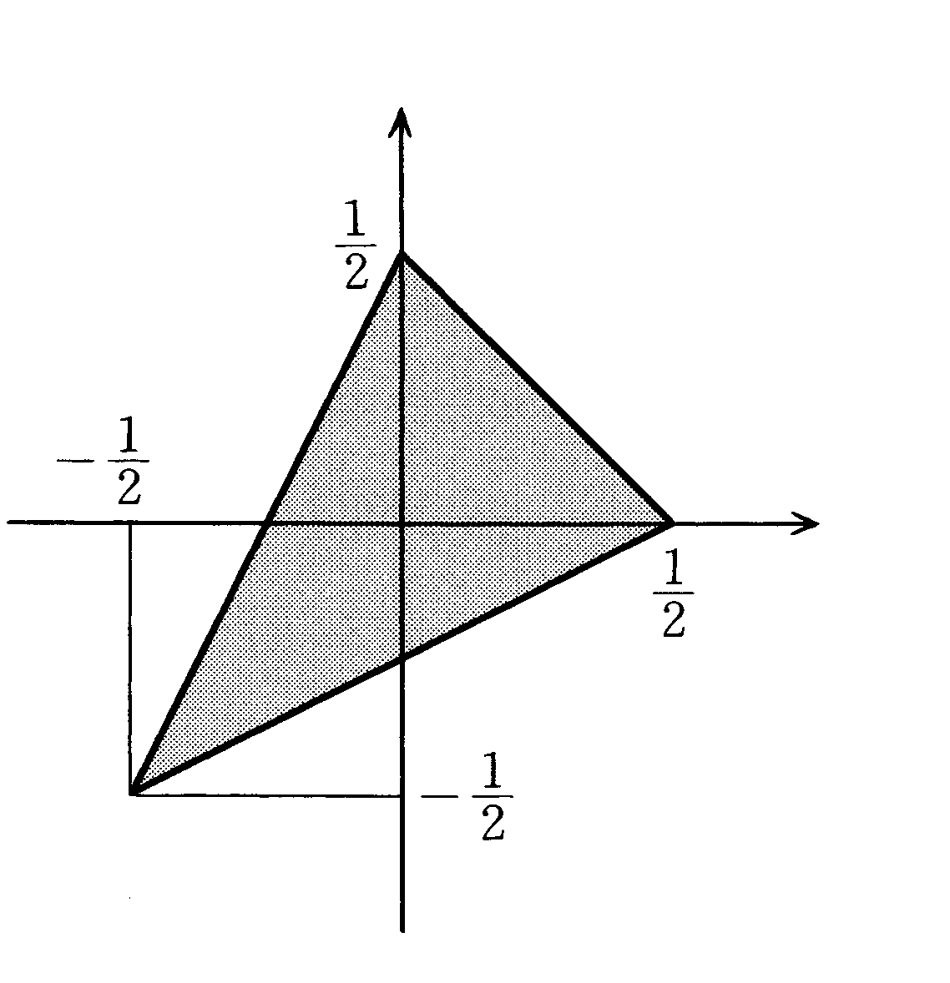
\includegraphics[width=0.42\textwidth]{figures/fig3.3.png}
  \figtitle{3.3}{动量映射的像（原书 p.107）}
\end{figure}

环面簇理论的核心，是用凸体 $f(M)$\footnote{不过 $f(M)$ 在标准的“凸体 $\Longleftrightarrow$ 环面簇”对应（参见 [133]、[288]）中，并不是与 $M$ 对应的那个凸体本身。}的组合性质来描述 $M$ 的各种几何性质。这一理论具体例与应用丰富而重要，但基本上属于代数几何，本书不再多述。[133]、[288] 等有优秀的教科书。环面簇也有与代数几何不同的侧面，与许多领域相关。与等周不等式的关系参见 [54]，与奇点的关系参见 [137]。此外 [331] 等也很有意思。

% [原文 p.108]
\section{局部化与等变上同调}

\takeaway{Kirwan 的局部化定理：$\|f\|^2$ 的 Morse 理论把 $H^*_G(M;\Q)$ 按临界集 $C_{\beta,d}$ 的 Thom 空间分层，得到 $H^*_G(M;\Q)\cong\bigoplus_{\beta,d}H^{*-2d}_G(C_{\beta,d};\Q)$；于是限制映射 $H^*_G(M;\Q)\to H^*_G(f^{-1}(0);\Q)$ 满射。}

本节解说 Kirwan [200] 等人关于辛商上同调的结果。先定义等变上同调。众所周知，对任意的紧李群 $G$，存在 $G$ 自由作用（free，即若对某个 $g\in G$、$x\in X$ 有 $gx=x$，则 $g=1$）的可缩空间 $EG$，且在等变同伦同值的意义下唯一。（若 $G\subset O(k)$，则可置 $X_n=G\backslash O(n+k)/O(n)$，取归纳极限 $\varinjlim X_n$。$O(k)\subset O(n+k)$ 通过左乘作用在 $X_n$ 上。）

设 $M$ 是 $G$ 作用的空间，把 $M\times EG$ 关于 $G$ 的对角作用 $g(x,y)=(gx,gy)$ 的商空间记作 $M\times_GEG$。（这称为 \textbf{Borel 构造}（Borel construction）。）

\begin{definition}{3.47}
  对可换环 $R$，$M$ 的\textbf{等变上同调}（equivariant cohomology）$H^*_G(M;R)$ 指 $M\times_GEG$ 的上同调 $H^*(M\times_GEG;R)$。
\end{definition}

若 $G$ 在 $M$ 上的作用是自由的，则 $H^*_G(M;R)$ 与商空间 $M/G$ 的上同调一致。

% [Tutor Note: 更准确地说，$H^*_G(M;R)$ 是 $H^*_G(\text{pt};R)=H^*(BG;R)$ 上的模；$G$ 自由作用时 $M\times_GEG\to M/G$ 是纤维为 $EG$ 的纤维化，其底空间的上同调正是 $H^*(M/G;R)$，这就是“一致”的含义。$H^*_G(\text{pt};R)$ 一般不是 $R$，故等变上同调不是普通上同调的简单推广。]

等变上同调给出从 $G$ 作用的空间的范畴出发的反变函子（contravariant functor）。普通上同调的许多性质在等变上同调中也成立。哪些成立，留给读者思考。

本节的主定理是下面的定理。

\begin{theorem}{3.48（Kirwan [200]）}
  设紧连通李群 $G$ 在紧辛流形 $(M,\omega_M)$ 上有哈密顿作用，$f\colon M\to\mathfrak{g}^*$ 是其动量映射。此时，嵌入所诱导的映射
  \[
    i^*\colon H^*_G(M;\Q)\to H^*_G(f^{-1}(0);\Q)
  \]
  是满射。（当 $0$ 是 $f$ 的正则值时，$H^*_G(f^{-1}(0);\Q)$ 就是辛商 $M/\!/G=f^{-1}(0)/G$ 的上同调。）
\end{theorem}

先极简地复习一点李群的术语。紧连通李群 $G$ 中存在极大环面 $\T\subset G$，$G$ 的任意可换子群都与 $\T$ 的某个子群共轭

% [原文 p.109]
设 $N\T=\{g\in G\mid g\T g^{-1}=\T\}$，则 $N\T/\T$ 是有限群 $W$。称 $W$ 为\textbf{Weyl 群}（Weyl group）。设 $\mathfrak{t}$ 是 $\T$ 的李代数。称 $W$ 在 $\mathfrak{t}$ 上共轭作用的基本区域为\textbf{Weyl 房}（Weyl chamber），记作 $\mathfrak{t}^+$。$\mathfrak{t}^+$ 是由有限个过原点的超平面围成的凸多面体，Weyl 群的作用由关于这些面的镜映（reflection）生成。

回到定理 3.48 的证明。定义 $h\colon M\to\R$ 为 $h(p)=\|f(p)\|^2$。$h$ 的 Morse 理论是证明定理 3.48 的主要工具。先确定临界点集 $\operatorname{Cr}(h)$。

在 $\mathfrak{g}$ 上取正定不变内积，把 $\mathfrak{g}$ 与 $\mathfrak{g}^*$ 等同起来。对 $\beta\in\mathfrak{g}$，定义 $f_\beta\colon M\to\R$ 为 $f_\beta(p)=f(p)(\beta)$。$f_\beta$ 是 $\beta$ 生成的 $\R$ 作用的动量映射。在 $M$ 上选好 $G$ 不变的黎曼度量 $g_M$ 与近复结构 $J_M$（引理 3.32）。

对 $\beta\in\mathfrak{t}$，把 $\{\exp(t\beta)\mid t\in\R\}$ 的闭包记作 $\T_\beta$。$\T_\beta$ 是环面。置 $\operatorname{Fix}(\T_\beta)=\{p\in M\mid\forall g\in\T_\beta,\ gp=p\}$。

\begin{lemma*}{3.49}
  $f_\beta$ 是 Bott–Morse 函数，且 $\operatorname{Cr}(f_\beta)=\operatorname{Fix}(\T_\beta)$。进一步，$T_p\operatorname{Fix}(\T_\beta)$ 关于 $J_M$ 不变。
\end{lemma*}

\begin{proof}
  与定理 3.14 相似，故简略记述。设 $p\in\operatorname{Fix}(\T_\beta)$。把 $T_pM$ 看作 $\T_\beta$ 的表示空间，则子空间 $T_p\operatorname{Fix}(\T_\beta)$ 对应平凡表示的部分。也就是说，法丛的纤维 $N_p\operatorname{Fix}(\T_\beta)$ 不含平凡表示。因此 $N_p\operatorname{Fix}(\T_\beta)$ 分解为实 2 维表示的直和 $\bigoplus\C_{\alpha_i}$。这里 $\alpha_i\colon\T_\beta\to U(1)$。由于 $J_M,\omega_M,g_M$ 是 $\T_\beta$ 不变的，$\C_{\alpha_i}$ 是 $J_M$ 不变的，即 $T_p\operatorname{Fix}(\T_\beta)$ 也是 $J_M$ 不变的。

  $X_i,Y_i$ 取为 $\C_{\alpha_i}$ 的（$\R$ 上的）基，并令 $Y_i=J_MX_i$。设 $\alpha_i$ 的微分把 $\beta$ 映为 $\sqrt{-1}\lambda_i$，则与 (3.5) 同样可证
  \[
    \operatorname{Hess}f_\beta(X_i,X_i)=\operatorname{Hess}f_\beta(Y_i,Y_i)=\lambda_i,\qquad
    \operatorname{Hess}f_\beta(X_i,Y_i)=0.
  \]
  由此得到本引理。
\end{proof}

% [Tutor Note: 证明里出现的 $\lambda_i$ 与 (3.5) 中的 $\lambda_i$ 是同一个量：$\T_\beta$ 在 $\C_{\alpha_i}$ 上以权重 $\lambda_i$ 旋转，故 $f_\beta$ 在该 2 维方向上的二次项恰为 $\lambda_i(x_i^2+y_i^2)$，Hessian 的两个特征值都是 $\lambda_i$、交叉项为 0。正因如此 $\operatorname{Cr}(f_\beta)$ 的负惯性指数可以直接由权重读出。]

\begin{definition}{3.50}
  $Z_\beta=\{p\in\operatorname{Fix}(\T_\beta)\mid f_\beta(p)=\|\beta\|^2\}$。
\end{definition}

\begin{proposition*}{3.51}
  (1) 在 $Z_\beta$ 上 $h\ge\|\beta\|^2$，且等号成立与 $p\in f^{-1}(\beta)\cap Z_\beta$ 或 $p\in f^{-1}(-\beta)\cap Z_{-\beta}$ 等价。

  (2) $\operatorname{Cr}(h)=\sum_\beta G\cdot(f^{-1}(\beta)\cap Z_\beta)$。

  (3) 使 $f^{-1}(\beta)\cap Z_\beta\neq\emptyset$ 的 $\beta\in\mathfrak{t}$ 只有有限个。
\end{proposition*}

% [原文 p.110]
证明之前先举一例。

\begin{example}{3.52}
  考虑例 3.37、3.46 中的 $M$、$T^2=G$。使 $f^{-1}(\beta)\cap Z_\beta\neq\emptyset$ 的 $\beta$ 是三角形 3 条边上从原点所引垂线的垂足 $\beta_1,\beta_2,\beta_3$ 与 3 个顶点 $\beta_4,\beta_5,\beta_6$。$\T_{\beta_1},\T_{\beta_2},\T_{\beta_3}$ 的李代数分别由 $A_1+A_2$、$A_1-2A_2$、$A_2-2A_1$ 生成。关于齐次坐标 $[z_0:z_1:z_2]$，$\operatorname{Fix}(\T_{\beta_1})$、$\operatorname{Fix}(\T_{\beta_2})$、$\operatorname{Fix}(\T_{\beta_3})$ 分别由 $z_0=z_1=0$ 或 $z_2=0$，$z_0=z_2=0$ 或 $z_1=0$，$z_1=z_2=0$ 或 $z_0=0$ 给出。$Z_{\beta_1},Z_{\beta_2},Z_{\beta_3}$ 分别是 $z_2=0$、$z_1=0$、$z_0=0$，它们是 $\operatorname{Fix}(\T_{\beta_i})$ 与以 $\beta_i$ 为重心的边的 $f$ 原像之交。$Z_{\beta_1}\cap f^{-1}(\beta_1)$、$Z_{\beta_2}\cap f^{-1}(\beta_2)$、$Z_{\beta_3}\cap f^{-1}(\beta_3)$ 分别由 $|z_0|=|z_1|$ 且 $z_2=0$，$2|z_0|^2=3|z_2|^2$ 且 $z_1=0$，$2|z_1|^2=3|z_2|^2$ 且 $z_0=0$ 给出，都是 $S^1$。
\end{example}

\begin{figure}[htbp]
  \centering
  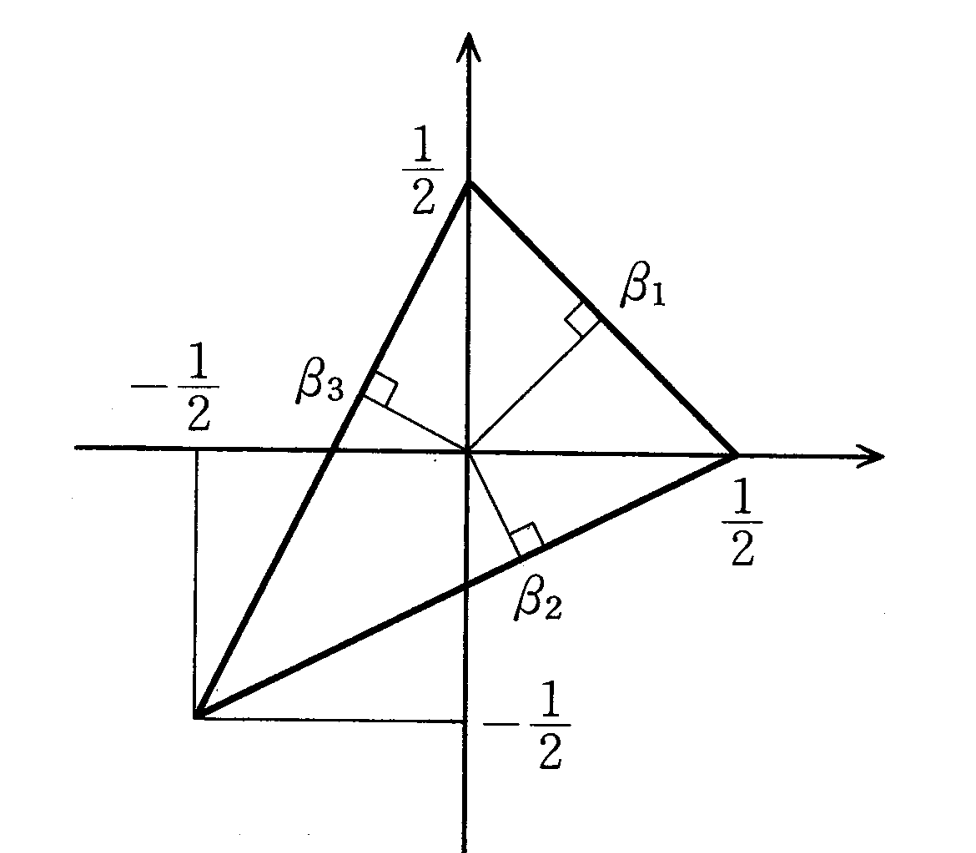
\includegraphics[width=0.44\textwidth]{figures/fig3.4.png}
  \figtitle{3.4}{（原书 p.110）}
\end{figure}

\begin{proof}[命题 3.51 的证明]
  (1) 若 $p\in Z_\beta$，则 $\sqrt{h(p)}=\|f(p)\|\ge|f(p)(\beta)|/\|\beta\|=\|\beta\|$。等号成立与 $\|f(p)\|\,\|\beta\|=|f(p)(\beta)|$ 等价，而这与 $f(p)=\beta$ 或 $f(p)=-\beta$ 等价。

  (2) 设 $p\in f^{-1}(\beta)\cap Z_\beta$，则由定义 $d_ph=2\langle d_pf,f(p)\rangle=2\langle d_pf,\beta\rangle=2d_pf_\beta=0$。由于 $h$ 是 $G$ 不变的，$G\cdot(f^{-1}(\beta)\cap Z_\beta)\subset\operatorname{Cr}(h)$。反之，设 $p\in\operatorname{Cr}(h)$。$\mathfrak{g}$ 的任意元素经共轭作用可移到 $\mathfrak{t}$ 的元素，故不妨设 $f(p)\in\mathfrak{t}$

% [原文 p.111]
  不妨设 $f(p)=\beta$。此时 $0=f_\beta h=2\langle d_pf,\beta\rangle=2d_pf_\beta$，故 $p\in\operatorname{Cr}(f_\beta)=\operatorname{Fix}(\T_\beta)$。于是由 (1)，$p\in Z_\beta$。即 $p\in f^{-1}(\beta)\cap Z_\beta$。

  (3) $f(M)$ 紧。又对 $\beta(\tau)$，$\tau\in[0,1]$，若 $\T_{\beta(\tau)}$ 的维数一定，则 $\T_{\beta(\tau)}$ 本身不依赖于 $\tau$。由这两点，存在有限集 $\beta(1),\dots,\beta(k)$，使对 $\beta\in f(M)$，$\T_\beta$ 与某个 $\T_{\beta(i)}$ 一致。

  设 $\mathfrak{t}_{\beta(i)}$ 是 $\T_{\beta(i)}$ 的李代数，则 $f$ 与正交射影 $\mathfrak{g}\to\mathfrak{t}_{\beta(i)}$ 的合成 $M\to\mathfrak{t}_{\beta(i)}$ 在 $\operatorname{Fix}(\T_\beta)$ 上的微分为 0。事实上，对 $\beta\in\mathfrak{t}_{\beta(i)}$、$p\in\operatorname{Fix}(\T_{\beta(i)})$ 有 $\langle d_pf,\beta\rangle=d_pf_\beta$，而 $f_\beta$ 是 $\R\subset\T_{\beta(i)}$ 的作用的动量映射，故 $d_pf_\beta=0$。

  因此，$f(\operatorname{Fix}(\T_{\beta(i)}))\cap\mathfrak{t}_{\beta(i)}$ 的元素个数不超过 $\operatorname{Fix}(\T_{\beta(i)})$ 的连通分量数，特别地 $f(\operatorname{Fix}(\T_{\beta(i)}))\cap\mathfrak{t}_{\beta(i)}$ 是有限集。由此得到 (3)。
\end{proof}

\begin{definition}{3.53}
  考虑 $\{\beta\in\mathfrak{t}^+\mid f^{-1}(\beta)\cap Z_\beta\neq\emptyset\}$，取其上的 Weyl 群 $W$ 作用的代表系，记作 $\mathbb{B}=\{\beta_1,\dots,\beta_b\}$。又置 $C_\beta=G\cdot f^{-1}(\beta)\cap Z_\beta$。
\end{definition}

命题 3.51 意味着
\[
  \operatorname{Cr}(h)=\bigcup_{\beta\in\mathbb{B}}C_\beta
  =\bigcup_{\beta\in\mathbb{B}}G\cdot(f^{-1}(\beta)\cap Z_\beta).
\]
又若 $\beta,\beta'$ 是 $\mathbb{B}$ 中互不相同的元素，则 $C_\beta\cap C'_{\beta'}=\emptyset$。至此 $\operatorname{Cr}(h)$ 就求出来了。

% [Tutor Note: (2) 中的和号写遍所有 $\beta$，但由 (3) 只有有限多个 $\beta$ 有贡献，故这是有限和。(1) 则说明 $f^{-1}(\beta)\cap Z_\beta$ 恰为 $h$ 在 $Z_\beta$ 上取最小值的点集；于是 $C_\beta=G\cdot(f^{-1}(\beta)\cap Z_\beta)$ 是 $\operatorname{Cr}(h)$ 的一个连通块，这就是 $\operatorname{Cr}(h)$ 的全部分类。]

$h$ 的 Morse 理论的困难之处在于：$h$ 未必是 Bott–Morse 函数。解决这一困难所用的，是下面的命题 3.54。

$Z_\beta$ 是 $\operatorname{Cr}(f_\beta)$ 的连通分量，故是光滑子流形（$f_\beta$ 是 Bott–Morse 函数）。设 $U(Z_\beta)$ 是 $Z_\beta$ 关于 $f_\beta$ 的不稳定流形（(3.9)）。$U(Z_\beta)$ 也是流形。

\begin{proposition}{3.54}
  (1) $G\cdot U(Z_\beta)$ 与 $C_\beta$ 的小邻域的交是光滑流形。

  (2) 若 $p\in C_\beta$，则 $T_p(G\cdot U(Z_\beta))$ 是 $\operatorname{Hess}_ph$ 的非负特征值所属特征空间之和。
\end{proposition}

证明稍后进行。$C_\beta$ 是 $f^{-1}(G\cdot\beta)\cap G\cdot U(Z_\beta)$。$G\cdot U(Z_\beta)$，

% [原文 p.112]
$G\cdot\beta$ 是光滑流形，但 $f\colon G\cdot U(Z_\beta)\to\mathfrak{g}$ 未必与 $G\cdot\beta$ 横截。例如 $\beta=0$ 的情形，$\operatorname{Cr}(0)=f^{-1}(0)$，一般不是流形。为说明命题 3.54 的意义，引入一些术语。

\begin{definition}{3.55}
  设 $h\colon M\to\R$ 是函数，$p\in\operatorname{Cr}(h)$。子流形 $U$ 称为 $p$ 的\textbf{不稳定中心流形}（unstable center manifold），是指下列条件 (1)、(2)、(3) 成立。

  (1) $U$ 关于 $\operatorname{grad}h$ 生成的 1 参数变换群不变。

  (2) $p\in U$。

  (3) $T_pU$ 与 $\operatorname{Hess}_ph$ 的非负特征空间之和一致。
\end{definition}

\textbf{稳定中心流形}（stable center manifold）、\textbf{中心流形}（center manifold）等概念可同样定义。\footnote{前者把 (3) 中的“非负”换成“非正”，后者换成“0”。}它们总是存在，但未必唯一。（以上参见例如 [375]。）

在 Bott–Morse 函数的情形，$p$ 的不稳定中心流形与含 $p$ 的临界子流形的不稳定部分流形一致。

在非 Bott–Morse 函数的一般情形，沿临界点集移动时，Hessian 的 0 特征值会变正或变负。因此不稳定中心子流形的维数会随点而变。

命题 3.54 意味着：在 $h$ 的情形，Hessian 的 0 特征值只会变正，负特征值的个数不变。由此，对临界点集的连通分量 $C_\beta$，存在“整体的不稳定中心子流形” $G\cdot U(Z_\beta)$。

开始证明命题 3.54。先从 (1) 开始。置 $\operatorname{Cent}(\beta)=\{g\in G\mid(\mathrm{ad}\,g)\beta=\beta\}$。换言之，$\operatorname{Cent}(\beta)$ 是 $\T_\beta$ 的中心化群（centerizer）。由定义，若 $g\in\operatorname{Cent}(\beta)$，则 $gU(Z_\beta)=U(Z_\beta)$。下面的引理说的是，其逆对属于 $Z_\beta\cap f^{-1}(\beta)$ 近旁的 $p$ 成立。

\begin{lemma*}{3.56}
  设 $p\in Z_\beta\cap f^{-1}(\beta)$。

  (1) 若 $gp\in U(Z_\beta)$，则 $g\in\operatorname{Cent}(\beta)$。

  (2) 若 $V\in\mathfrak{g}$，$V(p)\in T_p(U(Z_\beta))$，则 $V\in\operatorname{Lie}(\operatorname{Cent}(\beta))$。
\end{lemma*}

% [原文 p.113]
\begin{proof}
  (1) $gp\in U(Z_\beta)$ 且 $f_\beta$ 在 $Z_\beta$ 上等于 $\|\beta\|^2$，故 $f_\beta(gp)\ge\|\beta\|^2$。另一方面，$\|f(gp)\|^2=\|f(p)\|^2=\|\beta\|^2$。因此 $f(gp)=\beta$。即 $g\beta=\beta$。

  (2) 设 $\exp(tV)$ 是 $V$ 生成的 1 参数变换群。存在 $W$ 使
  \[
    f(\exp(tV)p)=\beta+t[V,\beta]+t^2W+O(t^3)
  \]
  （用到定义 3.1 (2)）。$\|f(gp)\|$ 不依赖于 $g\in G$。故 $\|\beta+t[V,\beta]+t^2W+O(t^3)\|=\|\beta\|$。于是 $\langle\beta,[V,\beta]\rangle=-\langle[V,\beta],\beta\rangle=0$，从而
  \begin{equation}
    2\langle\beta,t^2W\rangle=-t^2\|[V,\beta]\| \tag{3.20}
  \end{equation}
  另一方面，
  \begin{equation}
    \begin{aligned}
      f_\beta(\exp(tV)p)&=\|\beta\|^2+t\langle[V,\beta],\beta\rangle+t^2\langle W,\beta\rangle+O(t^3)\\
      &=\|\beta\|^2+t^2\langle W,\beta\rangle+O(t^3)
    \end{aligned}
    \tag{3.21}
  \end{equation}
  由 (3.21) 与 $V(p)\in T_p(U(Z_\beta))$ 得 $\langle W,\beta\rangle\ge0$。故由 (3.20)，$[V,\beta]=0$。即 $V\in\operatorname{Lie}(\operatorname{Cent}(\beta))$。
\end{proof}

回到命题 3.54 (1) 的证明。考虑 $\operatorname{Cent}(\beta)$ 在 $G\times U(Z_\beta)$ 上的作用 $h(g,p)=(gh^{-1},hp)$，把商空间记作 $G\times_{\operatorname{Cent}(\beta)}U(Z_\beta)$。这是流形。考察映射 $G\times_{\operatorname{Cent}(\beta)}U(Z_\beta)\to G\cdot U(Z_\beta)$。由引理 3.56 (1)，这个映射在 $1\times C_\beta$ 的近旁是同胚。进一步，由引理 3.56 (2)，这个映射在 $1\times C_\beta$ 的近旁是微分同胚。(1) 由此可得。

来证 (2)。若 $g\in G$，$p\in U(Z_\beta)$，则 $\|f(gp)\|=\|f(p)\|\ge f_\beta(p)/\|\beta\|\ge\|\beta\|$（最后的等号由 $p\in U(Z_\beta)$ 与 $Z_\beta$ 上 $f_\beta=\|\beta\|^2$ 得到）。也就是说，$h$ 在 $G\cdot U(Z_\beta)$ 上的限制在 $C_\beta$ 处取最小值 $\|\beta\|^2$。因此，只需对 $p\in C_\beta$ 证明 $\operatorname{Hess}_ph$ 在 $T_p(G\cdot U(Z_\beta))$ 的 $g_M$ 正交补空间 $T_p(G\cdot U(Z_\beta))^{\perp}$ 上负定。

只需考虑 $p\in f^{-1}(\beta)\cap Z_\beta$ 的情形。由引理 3.49 及其证明，$T_p(G\cdot U(Z_\beta))$ 关于 $J_M$ 不变。因此 $\omega_M$ 在 $T_p(G\cdot U(Z_\beta))$ 上非退化。进一步，$T_p(G\cdot U(Z_\beta))^{\perp}$ 是 $T_p(G\cdot U(Z_\beta))$ 关于 $\omega_M$ 的正交补空间。

设 $V\in T_p(G\cdot U(Z_\beta))^{\perp}$，$W\in\mathfrak{g}$，则 $W(p)\in T_p(G\cdot U(Z_\beta))$，故

% [原文 p.114]
$(d_pf)(V)(W)=\omega_M(W(p),V)=0$。即 $(d_pf)(V)=0$。因此存在 $a\in\mathfrak{g}$ 使
\[
  f(\exp(tV)p)=\beta+t^2a+O(t^3).
\]
由 $h=\|f\|^2$，
\begin{equation}
  h(\exp(tV)p)=\|\beta\|^2+2t^2\langle a,\beta\rangle+O(t^3) \tag{3.22}
\end{equation}
另一方面，
\begin{equation}
  f_\beta(\exp(tV)p)=\|\beta\|^2+t^2\langle\beta,a\rangle+O(t^3) \tag{3.23}
\end{equation}
由于 $T_p(G\cdot U(Z_\beta))^{\perp}$ 与 $T_p(G\cdot U(Z_\beta))$ 正交，$\operatorname{Hess}_pf_\beta$ 在 $T_p(G\cdot U(Z_\beta))^{\perp}$ 上负定。于是由 (3.22)、(3.23) 可知，$\operatorname{Hess}_ph$ 在 $T_p(G\cdot U(Z_\beta))^{\perp}$ 上负定。

至此命题 3.54 的证明完成。\hfill$\blacksquare$

\begin{definition}{3.57}
  \[
    Z_{\beta,d}=\{p\in Z_\beta\mid \operatorname{Hess}_pf_\beta \text{ 的负特征空间是实 }2d\text{ 维}\},
  \]
  \[
    C_{\beta,d}=\{p\in C_\beta\mid \dim T_p(G\cdot U(Z_\beta))^{\perp}=2d\}.
  \]
\end{definition}

% [Tutor Note: $C_{\beta,d}$ 的定义式里的 $\dim T_p(G\cdot U(Z_\beta))^{\perp}$ 就是 $h$ 在 $p$ 处的负惯性指数；由命题 3.54 (2)，它与 $\operatorname{Hess}_pf_\beta$ 的负特征空间维数一致，故 $C_{\beta,d}$ 正是 $C_\beta$ 中负指数恰为 $2d$ 的部分。这一分层是定理 3.58 中 $\bigoplus_{\beta,d}$ 的来源。]

由引理 3.56，注意下式 (3.24) 成立。
\begin{equation}
  H^*_G(C_{\beta,d};\Q)\simeq H^*_{\operatorname{Cent}(\beta)}(f^{-1}(\beta)\cap Z_{\beta,d};\Q). \tag{3.24}
\end{equation}

定理 3.17、3.23 的类似物是下面的定理。

\begin{theorem}{3.58}
  嵌入 $C_\beta\to M$ 诱导下列同型：
  \[
    H^k_G(M;\Q)\simeq\bigoplus_{\beta,d}H^{k-2d}_G(C_{\beta,d};\Q).
  \]
\end{theorem}

定理的结论可表述为：$h$ 在 $\Q$ 上等变完全（equivariantly perfect over $\Q$）。

\begin{remark}{3.59}
  定理 3.58 意味着：$M$ 的整体性质（上同调）在群作用存在时，被局部化到群不动点附近的性质上。这一原理还有许多其他应用（例如参见 [135]）。
\end{remark}

由于 $C_{0,0}=f^{-1}(0)$，定理 3.48 可由定理 3.58 得到。定理 3.58 的证明是本节的剩余目标。设 $\varphi_t$ 是 $\operatorname{grad}h$ 生成的 1 参数变换群。

% [原文 p.115]
\begin{lemma}{3.60}
  $\lim_{t\to\infty}\varphi_t(p)$、$\lim_{t\to-\infty}\varphi_t(p)$ 对任意的 $p$ 都收敛。
\end{lemma}

$h$ 未必是 Bott–Morse 函数，故引理 3.60 不能由引理 3.19 推出，但可用命题 3.54 证明（参见 [200]）。应用上重要的是 $h$ 为实解析函数的情形，此时由注 3.21 也可得出。

\begin{definition}{3.61}
  $S(C_{\beta,d})=\{p\mid \lim_{t\to-\infty}\varphi_t(p)\in C_{\beta,d}\}$。
\end{definition}

把 $G\cdot U(Z_{\beta,d})$ 的法丛限制到 $C_{\beta,d}$ 上，记作 $N^-(C_{\beta,d})$。

\begin{lemma}{3.62}
  $S(C_{\beta,d})\to C_{\beta,d}$，$p\mapsto\lim_{t\to-\infty}\varphi_t(p)$ 连同 $G$ 的作用在内，与 $N^-(C_{\beta,d})\to C_{\beta,d}$ 微分同胚。
\end{lemma}

引理 3.62 是引理 3.18 的类似物，用命题 3.54（特别是 (2)）证明。证明省略（参见 [200]）。

$h$ 的临界值只有有限个。设 $r_0=0<r_1<\cdots<r_m$。置
\[
  \mathfrak{X}_k=\bigcup_{h(C_{\beta,k})\le r_k}S(C_{\beta,k}).
\]
引理 3.22 的类似物可由引理 3.60 证明，故 $\mathfrak{X}_k$ 是闭集。$\mathfrak{X}_k$ 是其近旁的收缩核，这可用命题 3.54 证明。因此确定了 $S_*(M)$ 的滤过 $S_*(\mathfrak{X}_k)$。

\begin{remark}{3.63}
  用滤过 $S_*(\mathfrak{X}_k)$，可确定一个谱序列：其 $E_2$ 项是定理 3.58 的右端，收敛到 $M$ 的上同调（定理 3.58 的左端）（定理 3.17 的类似物\footnote{不过稳定流形与不稳定流形是反过来的。}）。这个谱序列退化，就是定理 3.58。不过，以下不使用谱序列的语言。
\end{remark}

考虑长正合列
\[
  \to H^\ell_G(\mathfrak{X}_k(M),\mathfrak{X}_{k-1}(M);\Q)\to H^\ell_G(\mathfrak{X}_k(M);\Q)
  \to H^\ell_G(\mathfrak{X}_{k-1};\Q)\to
\]
由引理 3.62、切除同型以及等变 Thom 同型（下面马上说明），
\begin{equation}
  H^\ell_G(\mathfrak{X}_k(M),\mathfrak{X}_{k-1}(M);\Q)
  \simeq\bigoplus_{h(C_{\beta,d})=r_k}H^{\ell-2d}_G(C_{\beta,d};\Q). \tag{3.25}
\end{equation}

% [原文 p.116]
于是，由下面的引理，定理 3.58 的证明即完成。

\begin{lemma*}{3.64}
  $i^*\colon H^\ell_G(\mathfrak{X}_k(M),\mathfrak{X}_{k-1}(M);\Q)\to H^\ell_G(\mathfrak{X}_k(M);\Q)$ 是单射。
\end{lemma*}

\begin{proof}
  把 (3.25) 与嵌入 $C_{\beta,d}\to\mathfrak{X}_k(M)$ 所导出的映射合成，得到
  \begin{equation}
    H^{\ell-2d}_G(C_{\beta,d};\Q)\to H^\ell_G(C_{\beta,d};\Q). \tag{3.26}
  \end{equation}
  只需证明 (3.26) 是单射。由向量丛 $N^-(C_{\beta,d})\to C_{\beta,d}$ 得到 $N^-(C_{\beta,d})\times_GEG\to C_{\beta,d}\times_GEG$。其 Euler 类
  \begin{align*}
    e(N^-(C_{\beta,d})\times_GEG)
    &\in H^{2d}\bigl(N^-(C_{\beta,d})\times_GEG,(N^-(C_{\beta,d})-C_{\beta,d})\times_GEG;\Z\bigr)\\
    &=H^{2d}_G\bigl(N^-(C_{\beta,d}),N^-(C_{\beta,d})-C_{\beta,d};\Z\bigr)
  \end{align*}
  称为\textbf{等变 Euler 类}（equivariant Euler class）。等变 Thom 同型由与等变 Euler 类的杯积定义。把 $e(N^-(C_{\beta,d})\times_GEG)$ 经限制映射移到 $H^{2d}_G(N^-(C_{\beta,d});\Z)$ 中，所得仍用同一记号表示。$N^-(C_{\beta,d})$ 与 $C_{\beta,d}$ 同伦等价，故等变 Euler 类给出 $C_{\beta,d}$ 的上同调类。把这个元素记作 $e(\beta,d)$。与 $e(\beta,d)$ 的杯积就是映射 (3.26)。由 (3.24)，可把 $e(\beta,d)$ 看作属于 $H^{2d}_{\T_\beta}(f^{-1}(\beta)\cap Z_{\beta,d};\Q)$。因此，由下面的引理 3.65（据 Atiyah–Bott [20]）可得引理 3.64。
\end{proof}

\begin{lemma*}{3.65}
  \[
    H^{k-2d}_{\operatorname{Cent}(\beta)}(f^{-1}(\beta)\cap Z_{\beta,d};\Q)
    \to H^k_{\operatorname{Cent}(\beta)}(f^{-1}(\beta)\cap Z_{\beta,d};\Q),\qquad
    x\mapsto x\cup e(\beta,d)
  \]
  是单射。
\end{lemma*}

\begin{proof}
  存在 $\operatorname{Cent}(\beta)$ 的有限覆盖 $\widetilde{\operatorname{Cent}}(\beta)$，使 $\T_\beta$ 的原像 $\tilde{\T}_\beta$ 是直积因子，且 $\widetilde{\operatorname{Cent}}(\beta)\simeq\tilde{\T}_\beta\times G'$。由于在上同调中取有理系数，不妨假定 $\widetilde{\operatorname{Cent}}(\beta)=\operatorname{Cent}(\beta)$（这是必须取有理系数的唯一之处）。$EG=E\tilde{\T}_\beta\times EG'$。把向量丛
  \begin{equation}
    N^-(C_{\beta,d})\times_{G'}EG'\to(f^{-1}(\beta)\cap Z_{\beta,d})\times_{G'}EG' \tag{3.27}
  \end{equation}
  写作 $\pi\colon\xi\to X$。(3.27) 上有环面 $\T=\tilde{\T}_\beta$ 作用，其在纤维上的限制由定义不含平凡不可约成分。因此引理 3.65 归结为下面的引理 3.66。

% [Tutor Note: 有理系数正是在此处不可省：把 $\operatorname{Cent}(\beta)$ 换成有限覆盖后，$\T_\beta$ 才成为直积因子。这一步若用整数系数，则 $H^*(\text{pt};\Z)$ 中的挠元会破坏单射性。这正是定理 3.23 能对整数系数成立、而定理 3.48 一般只能对 $\Q$ 系数成立的原因。]
\end{proof}

\begin{lemma*}{3.66}
  设 $\T$ 作用在向量丛 $\pi\colon\xi\to X$ 上，$X$ 上的 $\T$ 作用平凡，且 $\T$ 在纤维上的作用不含平凡不可约成分。

% [原文 p.117]
  此时，与等变 Euler 类 $e(\xi)\in H^*_\T(X;\Q)$ 的杯积诱导单射 $H^{k-2d}_\T(X;\Q)\to H^k_\T(X;\Q)$。
\end{lemma*}

\begin{proof}
  由于 $\T$ 在 $X$ 上的作用平凡，$X\times_\T E\T$ 是直积 $X\times(\CP^\infty)^{2b}$。这里 $2b=\dim\T$。于是由 Künneth 公式，
  \begin{equation}
    H^*_\T(X;\Q)\simeq H^*(X;\Q)\otimes H^*(\CP^\infty;\Q)^{\otimes b}. \tag{3.28}
  \end{equation}
  作不可约分解 $\xi_p\simeq\bigoplus_{j=1}^bL_j$（$L_j$ 的秩为 2）。考虑等变 Euler 类 $e(\xi)$ 在 $H_\T(p;\Q)\simeq H((\CP^\infty)^{2b};\Q)$ 中的限制 $e(\xi)_p$。$e(\xi)_p=e(L_1)\cup\cdots\cup e(L_b)$，而 $e(L_j)\in H_\T(p;\Q)$ 是 $\T\to U(1)$ 这一与 $L_j$ 对应的表示下，$H^2(\CP^\infty;\Q)\simeq H^2_{U(1)}(p;\Q)$ 的生成元之拉回。与 $L_j$ 对应的表示都不平凡，故 $e(L_j)\neq0$。$H_\T(p;\Q)$ 是多项式环，故与 $e(\xi)_p=e(L_1)\cup\cdots\cup e(L_b)$ 的杯积在 $H_\T(p;\Q)$ 上诱导单射。于是由 (3.28) 得到本引理。
\end{proof}

至此定理 3.48、3.58 的证明完成。\hfill$\blacksquare$

定理 3.23 可由定理 3.48 如下得出。注意：在此前的讨论中，必须取有理系数的只有引理 3.65 中用直积替换群的那一处。因此，在定理 3.23 的情形群是 $S^1$，故定理 3.48 对整数系数成立。

只需证明 $H^k(M;\Z)\to H^{k-\mu(R_i)}(R_i;\Z)$ 是满射。而由定理 3.58，$H_{S^1}(M;\Z)\simeq\bigoplus_iH^{k-\mu(R_i)}_{S^1}(R_i;\Z)$。又 $H_{S^1}(1\text{ 点};\Z)\simeq\Z[c]$，且
\[
  H(1\text{ 点};\Z)\simeq\frac{H_{S^1}(1\text{ 点};\Z)}{c\cup H_{S^1}(1\text{ 点};\Z)}.
\]
另一方面，
\[
  H^*_\T(R_i;\Z)\simeq H^*(X;\Z)\otimes H^*(\CP^\infty;\Z).
\]
因此
\[
  H_{S^1}(M;\Z)\simeq H^*(M;\Z)\otimes H^*(\CP^\infty;\Z)
\]

% [原文 p.118]
也是如此。由以上事实，定理 3.23 显然成立。

\begin{remark}{3.67}
  Atiyah–Bott [19] 对黎曼面上平坦向量丛的模空间 $\mathcal{M}(\Sigma,E)$ 的情形应用定理 3.58，求出了其 Betti 数（Betti number）等。更准确地说，[19]、[20] 先于 Kirwan 的 [200]；看到 Atiyah–Bott 的结果并将其一般化的，就是 [200]。
\end{remark}

定理 3.48、3.58 只叙述了等变上同调作为可换群的结构。与杯积的关系也有人研究，由 Duistermaat–Heckman [85] 开端，Witten [394]、Jeffrey–Kirwan [189]、[190] 等考察了许多内容。积结构的研究被应用于共形场论中 Verlinde 公式的另一证明等。这些都是非常重要的结果，此处从略。除上面举出的原始论文外，[24]、[169] 等也可参考。

此外，与等变上同调和动量映射相关的话题，还有 Mathai–Quillen 流派的表述（Mathai–Quillen formalism [247]）以及 BRST 上同调\footnote{[37] 是最初的论文，但它是物理文献。对数学专家较易读的文献可举例如 [66]。}。

本书没有讲述，但对超凯勒流形（hyper Kähler 流形），有超凯勒动量映射（hyper Kähler moment map）这一类似概念。它发端于 [180] 附近，产生了 [21]、[225]、[227] 等许多应用。

对哈密顿力学系统对称性的研究，有着上溯到 Lagrange 与 Euler 的悠久传统；本书关于辛商的叙述，偏重于代数几何与量子场论附近的部分。希望读者用例如 [244] 以及那里大量引用的文献来补充。

\chapterreview{本章的地位是双重的。一方面，它暂时放下第 2 章的伪全纯曲线技术，回到辛几何最古典的构造手段——群作用；另一方面，它又是此后各章的例子库：加权射影空间、环面簇、平坦联络的模空间，其辛结构都从这里取得。辛商的构造可以说是“从局部走向整体”这一纲领在辛几何里最成功的一次兑现：对称性被一个函数（动量映射）记录，再由“除以对称群”这一操作产生新的辛流形。

全章骨架清楚。§3.1 由定义 3.1 给出动量映射，用 Marsden–Weinstein 定理 3.4 说明辛形式可以沿正则值纤维下降到商上；§3.2 转入 $S^1$ 情形，把动量映射当作 Bott–Morse 函数处理，得到谱序列（定理 3.17）与退化定理 3.23，并以凸性定理 3.25 收尾；§3.3 讲复化：保持凯勒结构的哈密顿 $G$-作用能延拓为 $G_{\C}$ 的全纯作用，辛商于是同时是辛流形与复流形；§3.4 用等变上同调把前面的 Morse 论证提升为局部化定理，给出 Kirwan 的满射性（定理 3.48）与分解式（定理 3.58）。

最可用的结论有三条。定理 3.4 保证辛商 $M/\!/G=f^{-1}(0)/G$ 在 $0$ 为正则值且作用自由时确为辛流形，其辛形式由 $\pi^*\bar\omega=\omega|_{f^{-1}(0)}$ 唯一确定。定理 3.23 说明动量映射是“完全 Bott–Morse”的：$M$ 的同调由各临界子流形的同调完全决定，位移量恰是 Morse 指数。定理 3.58 把这一现象再提升为等变上同调的局部化，$M$ 的大范围信息由不动点附近的数据拼成。

须提醒几处易混。其一，动量映射不唯一，可以相差中心李代数的元素（命题 3.3、注 3.7），因而“稳定点集”也随动量映射的取法而变，§3.3 末尾用 $S^1$ 的 flip 说明了这一点。其二，定义辛商时假定了 $0$ 是正则值且作用自由；一旦退化，商不再是流形，须借助轨形（例 3.9）或不稳定中心流形（§3.4）处理。其三，$h=\|f\|^2$ 一般不是 Bott–Morse 函数，这是 §3.4 全部技术困难的来源，命题 3.54 用“Hessian 的零特征值只向正方向变”来弥补。

作者的处理偏重复几何与规范理论一侧：平坦联络模空间、环面簇、Kirwan 局部化三条线索贯穿全章，而辛商在 Floer 理论与量子上同调中的后续发展只以文献形式点到。这既与本书的写作年代有关，也提示读者：辛商是构造例子与计算不变量的工具，而不是终点。与后文的衔接有二：第 4 章用辛商刻画约化空间上的拉格朗日子流形与几何量子化；第 6 章把环面簇、加权射影空间当作 Gromov–Witten 不变量的检验场。若只读一遍，建议把定理 3.4、3.23、3.58 抄在一起对照——它们分别对应“存在”“计算”“局部化”三步，是本章的骨架。}

% CHUNK ch03 DONE
